% This is the Reed College LaTeX thesis template. Most of the work
% for the document class was done by Sam Noble (SN), as well as this
% template. Later comments etc. by Ben Salzberg (BTS). Additional
% restructuring and APA support by Jess Youngberg (JY).
% Your comments and suggestions are more than welcome; please email
% them to cus@reed.edu
%
% See https://www.reed.edu/cis/help/LaTeX/index.html for help. There are a
% great bunch of help pages there, with notes on
% getting started, bibtex, etc. Go there and read it if you're not
% already familiar with LaTeX.
%
% Any line that starts with a percent symbol is a comment.
% They won't show up in the document, and are useful for notes
% to yourself and explaining commands.
% Commenting also removes a line from the document;
% very handy for troubleshooting problems. -BTS

% As far as I know, this follows the requirements laid out in
% the 2002-2003 Senior Handbook. Ask a librarian to check the
% document before binding. -SN

%%
%% Preamble
%%
% \documentclass{<something>} must begin each LaTeX document
\documentclass[12pt, oneside, openright]{byuthesis}


\title{Consistent Mode Choices Across\\
Multiple Model Frameworks}
\author{Christopher Day}
\copyyear{2022}
\committeeMembers{Gregory S. Macfarlane, Chair

Grant G. Schultz

Gustavious P. Williams}
\keywords{four step model, discrete choice model, activity-based model, microsimulation tool, mode choice model, tour purpose, multinomial logit, latent class choice model}
\degree{Master of Science}
\doctype{thesis}
\department{Department of Civil and Construction Engineering}



	\usepackage{algorithm}
	\usepackage{algpseudocode}
	\usepackage{dsfont}
% End of CII addition
%%
%% End Preamble
%%
%

% Pandoc citation processing
\newlength{\cslhangindent}
\setlength{\cslhangindent}{1.5em}
\newlength{\csllabelwidth}
\setlength{\csllabelwidth}{3em}
\newlength{\cslentryspacingunit} % times entry-spacing
\setlength{\cslentryspacingunit}{\parskip}
% for Pandoc 2.8 to 2.10.1
\newenvironment{cslreferences}%
  {}%
  {\par}
% For Pandoc 2.11+
\newenvironment{CSLReferences}[2] % #1 hanging-ident, #2 entry spacing
 {% don't indent paragraphs
  \setlength{\parindent}{0pt}
  % turn on hanging indent if param 1 is 1
  \ifodd #1
  \let\oldpar\par
  \def\par{\hangindent=\cslhangindent\oldpar}
  \fi
  % set entry spacing
  \setlength{\parskip}{#2\cslentryspacingunit}
 }%
 {}
\usepackage{calc}
\newcommand{\CSLBlock}[1]{#1\hfill\break}
\newcommand{\CSLLeftMargin}[1]{\parbox[t]{\csllabelwidth}{#1}}
\newcommand{\CSLRightInline}[1]{\parbox[t]{\linewidth - \csllabelwidth}{#1}\break}
\newcommand{\CSLIndent}[1]{\hspace{\cslhangindent}#1}

\providecommand{\tightlist}{%
  \setlength{\itemsep}{0pt}\setlength{\parskip}{0pt}}


\begin{document}

\begin{abstract}
Every day individuals make a decision about which modes of transportation they should use. Predicting this behavior perfectly is impossible, however, there are ways to appoximating mode choice in transportation modeling. In this research we aim to increase the accuracy in predicting mode choice using transportation modeling software. Specifically we determine the significance of creating a consistent mode choice model between an activity-based model and a microsimulation tool. Oftentimes, the outputs of an activity-based model serve as the inputs to a microsimulation tool. Yet, the mode choice models betweeen these two software often vary significantly. Using ActivitySim as the activity-based model and BEAM as the microsimulation tool, we establish a consistent mode choice model within BEAM. We then model the mode choice decisions for agents in the Salt Lake City, Utah region. Their modal distributions and mode choice structures are compared to determine the effect of mode choice consistency. Interestingly, we find that a model that uses a consistent mode choice creates a modal distribution that aligns more closely with target shares. We also find that the introduction of path, person, and location variables in the mode choice utility equation helps better predict mode choice decisions. Further research is necessary in order to understand the effects of identical mode choice models between activity-based models and microsimulation tools.
\end{abstract}


\makefrontmatter % this stuff will be roman-numbered
\thesisbody

\hypertarget{introduction}{%
\chapter{Introduction}\label{introduction}}

\hypertarget{problem-statement}{%
\section{Problem Statement}\label{problem-statement}}

The advent of novel transport modes has challenged forecasters to develop new methods of capturing behavior and estimating service capabilities. The usage of bike share, an affordable and sustainable bike rent program, has been modeled countless times each with a different methodology (e.g., Hyland et al. (2018), Biehl, Ermagun, and Stathopoulos (2019), Cho and Shin (2022), W. Li and Kamargianni (2018), Welch, Gehrke, and Widita (2020), X. Zhou, Wang, and Li (2019), Song et al. (2019)). Forecasters are riddled with determining the best technique for understanding who uses e-scooters (public electric scooters) and in what locations they would be most effective (e.g, Zuniga-Garcia et al. (2022), Tuli, Mitra, and Crews (2021), Zhang et al. (2021), M. Lee et al. (2021), H. Lee et al. (2021), Hosseinzadeh et al. (2021)). (sentence on e-bikes). In general, forecasters have modeled micromobility (bike share, e-scooters, e-bikes) in many ways, yet few have attempted to model multiple novel modes simultaneously (e.g., Reck et al. (2021), Campbell et al. (2016), Lazarus et al. (2020), McKenzie (2019), Younes et al. (2020)). Ride hail and ride share, which allow users to hire a driver, behave differently than regular car modes. Given their unique nature, understanding their behavior and service capabilities is particularly challenging (e.g., Kang et al. (2021), Y. Li, Liu, and Xie (2020), Dong (2020), Dean and Kockelman (2021)). Forecasters have even attempted to understand the effects of autonomous vehicles, even though to date little to no data exists on fully-autonomous vehicles (e.g., Mo, Chen, and Zhang (2022), Wadud and Chintakayala (2021), F. Zhou et al. (2020)). New transport technologies are becoming more prominent each day, and equally so is the need to accurately capture their behavior.

Various efforts have been made to model novel transport modes accurately, but since methodologies are dissimilar with one another it remains difficult to determine the best approach. For example, some forecasters have chosen to model novel transport modes with an Activity-based Model (ABM), which use daily activity patterns as the central tool to model an individual's travel behavior (e.g., Xu, Mahmassani, and Chen (2019), Muhammad et al. (2019), Macfarlane, Lant, et al. (2021)). Other forecasters use Multi-agent Simulation (MAS) models, which focus on modeling the interactions between different agents, to understand new transport technologies (e.g., Shimizu, Akai, and Nishino (2013), Sánchez et al. (2019), Hörl et al. (2019)). \textbf{Many forecasters have modeled novel modes using a logit based regression analysis, which uses a function to understand characteristics of the modes (e.g., Welch, Gehrke, and Widita (2020), M. Lee et al. (2021), Dong (2020)).}(delete? -- logit regression is used in abm/mas models) Some chose a simpler approach, spatial analysis and geography data, to understand new transport technologies (e.g., Hyland et al. (2018), Cho and Shin (2022), Hosseinzadeh et al. (2021)). Forecasters have even attempted to use machine learning to better understand novel modes! (e.g., X. Zhou, Wang, and Li (2019)). With limited data on novel transport modes, the validity of the results from each approach can be difficult to verify.

\hypertarget{purpose-of-research}{%
\section{Purpose of Research}\label{purpose-of-research}}

In this paper we examine novel mode forecasts generated by different ABM and MAS mode choice combinations. By examining the ride hail service capabilities between each combination, we hope to understand which mode choice combinations is best, or if a best combination even exists. Since only limited data on novel mode usage exists, it seems logical to use a trial and error approach to determine the best way to model new transport technologies. Overall, this paper aims to give forecasters additional direction in how to model novel transport modes.

\hypertarget{literature-review}{%
\chapter{Literature Review}\label{literature-review}}

As discussed in the introduction, forecasters model novel transport modes using ABMs, MAS models, spatial analysis, machine learning, and more. Since our research mainly focuses on ABMs, MAS models, and the link between them both, understanding the other model frameworks is not within the scope of this project. For this reason, the following literature review outlines the strengths and weaknesses of ABMs and MAS models, the previous attempts to model novel transport modes with ABMs and MAS models, and the brief literature of those who have attempted to reconcile two modeling approaches within the same study.

\hypertarget{abm-introduction}{%
\section{ABM Introduction}\label{abm-introduction}}

ABMs are transportation models that construct daily activity patterns from behavioral choice models. They predict what activities are conducted, where those activities are conducted, the length and time of those activities, and the people involved in those activities. This detailed approach to modeling behavior allows forecasters to understand travel at a high level both spatially and temporally. According to Philip, Sreelatha, and George (2013), ABMs generate travel demand by first modeling activity demand. Understanding the idea that all travel is generated by activities is essential to accurately representing the way people travel. This link between activity and travel allows ABMs to model behavior especially well, which is particularly advantageous when modeling novel modes. Bowman (1998) also explains that ABMs have choice models that use utility theory and logit based regression to estimate behavior. These choice models accept an array of inputs relating to person, household, and regional data, to better capture the travel behavior of any particular region.

In addition to representing behavior accurately, another advantage to using ABMs is that there is modal consistency between trips on the same tour (e.g., Nayak and Pandit (2022), Hasnine and Nurul Habib (2021), Knapen et al. (2021), Gomes, CALDAS, and Pitombo (2021)). Nayak and Pandit (2022) explains that other existing models fail to consider the ``interrelationships among trips'' performed by the same individual on the same tour. For example, if you were to take your car to the gym, and then stop by the store on the way back home, wouldn't you also use your car to get from the store back to your home? Individuals will act similarly among trips of the same tour, and ABMs account for this nature tendency. Hasnine and Nurul Habib (2021) explains that tour based modeling is the core of ABMs; ``tackling'' every trip within a tour is essential to understanding how dynamics that exists between trips. Gomes, CALDAS, and Pitombo (2021) explains that trip-based models, unlike ABMs, disregard trip sequences, trips made by the same individual, and the relationship between trips and activities. Chaining trips of the same individual together, within the same tour, helps ensure modal consistency within models.

Knowing the advantages that ABMs provide when modeling travel behavior, many forecasters use ABMs to model the behavior and service capabilities of novel modes. For example, some new technologies that have been modeled with ABMs are car-sharing (e.g., Nguyen, Hoang, and Vu (2022), Q. Li et al. (2018)) and autonomous vehicles (e.g., Xu, Mahmassani, and Chen (2019), Vyas et al. (2019)). Nguyen, Hoang, and Vu (2022) modeled one-way car-sharing services with an ABM because the modal consistency between trips allowed them to track vehicle demand, pricing, and other parameters. Xu, Mahmassani, and Chen (2019) modeled privately-owned autonomous vehicles with an ABM as a way to better understand their impact on household travel patterns, including very large households. Macfarlane, Lant, et al. (2021) used an ABM to model on-demand wheelchair accessible microtransit vehicles. The ABM generated daily activity patterns for all individuals in the region, including those who were wheelchair dependent. With those plans they were able to simulate microtransit vehicle with a microsimulation tool, and process the results to understand service capabilities. Tzouras et al. (2022) conducted a quantitative study of ABMs for modeling e-scooters. They agreed that ABMs are an effective vehicle to describe the spatiotemporal variation in e-scooters, and novel modes in general. Muhammad et al. (2019) used an ABM to model bike share and even the concept of Mobility as a Service, which aims to make public transport a pay-per-service or monthly subscription. Many forecasters elect to use ABMs to model new transport technologies because of the behavioral representation and modal consistency they provide.

Although there are advantages to using ABMs to model novel modes, forecasters must consider the various weaknesses that exist when using ABMs. One of the biggest shortfalls within most ABMs is that travel times are averaged along travel links (e.g., RSG (2016), Mahmoudi et al. (2021)). For example, although Nguyen, Hoang, and Vu (2022) used an ABM to model one-way car sharing, they noted that it used the BPR function to estimate travel time. The BPR function is a regression function that estimates average travel time based on arrival flows. When using the BPR function to estimate smaller time intervals though, it becomes inconsistent. For this reason, Nguyen, Hoang, and Vu (2022) noted that it was more difficult to verify the service capabilities of the car-sharing modes. Similarly, on-demand microtransit vehicles should be modeled with variable wait time; the difference between a 4 minute wait and a 17 minute wait is significant when traveling. Overall, since travel time is a significant part of the mode choice utility, average travel time is a shortfall when modeling novel modes. \emph{talk about other weaknesses}

\hypertarget{methods}{%
\chapter{Methods}\label{methods}}

\hypertarget{overview}{%
\section{Overview}\label{overview}}

The approach to determine the effects of a consistent mode choice model between an activity-based model and a microsimulation tool required three main steps. The first step involved creating a test scenario that runs within the activity-based model ActivitySim and the microsimulation tool BEAM. Section \ref{mscen} explains this step including how the test scenario was created and how ActivitySim and BEAM were configured. The second step involved adjusting the internal code of BEAM to align the mode choice model with that of ActivitySim's. Section \ref{mbeam} explains the details behind the changes made to BEAM's default mode choice model to align more closely with that of ActivitySim's. Section \ref{mbeam} also describes the existing mode choice models within BEAM and how their components were altered. The last step was to calibrate the mode choice utility values within BEAM. Section \ref{mcalib} explains the details behind the validation and calibration of the mode choice parameters.

\hypertarget{mscen}{%
\section{Creating and Setting up the Test Scenario}\label{mscen}}

Designing a test scenario to use within ActivitySim and BEAM was essential to understanding and testing mode choice between models. This section explains the region that was used to model the test scenario. This section also explains how the input files needed to run both ActivitySim and BEAM were generated for the test scenario.

\hypertarget{test-scenario-region}{%
\subsection{Test Scenario Region}\label{test-scenario-region}}

The test scenario used in this research includes the approximate 2.1 million agents of the Salt Lake City, Utah, USA region. This region includes Box Elder, Davis, Salt Lake, Utah, and Weber counties. Figure \ref{fig:figregion} shows the 2881 Traffic Analysis Zones (TAZs) along with the five counties that make up the region of study.

This extensive region was selected for the following reasons:

\begin{enumerate}
\def\labelenumi{\arabic{enumi}.}
\tightlist
\item
  There is substantial data that exists for this region. Having sufficient data points for each of the TAZs was essential to creating the inputs to ActivitySim and BEAM. The majority of the data used for this research was gathered and shared by Wasatch Front Regional Council (WFRC), the Metropolitan Planning Organization (MPO) of Salt Lake county.
\item
  There currently exists a need to analyze this region with a microsimulation tool, such as BEAM. Specifically, the Utah Transit Authority (UTA) wishes to understand which specific sub regions in the Salk Lake area will best serve new on-demand transit vehicles. In some future research, this specific question will be answered. Along this this question, having a microsimulation model of a region will prove to be an effective method to answering multiple transportation service questions in the future. To date, only one previous analysis of this region has been conducted with the BEAM software (Lant 2021).
\item
  The size and population within the study area are comparable to other regions around the United States. This means that the work completed in this research may be useful to other cities besides Salt Lake City.
\item
  The project researchers live in this region, and therefore have real life knowledge of how transportation works in the region. This allows the researchers to compare the results of the models with their own experiences, hopefully providing extra verification.
\end{enumerate}

Overall, the Salt Lake City, Utah region proved to be an effective location for this mode choice analysis research. After selecting the region of study, the next steps involved setting up and running ActivitySim.

\hypertarget{setting-up-and-running-activitysim}{%
\subsection{Setting up and Running ActivitySim}\label{setting-up-and-running-activitysim}}

Setting up and running ActivitySim for the Salt Lake region was based off example scenarios presented by ActivitySim (ActivitySim 2021). The entire process for setting up the activity-based model for this region is explained in the research done by Lant (2021). The research done by Lant (2021) was the basis to the work completed in this project.

However, a brief explanation of the setup of the activity-based model is explained in Section \ref{asiminput}. The two main steps behind creating an activity-based model for the Salt Lake region was creating corresponding input files and calibrating and validating the results.

\hypertarget{asiminput}{%
\subsubsection{Creating Input Files}\label{asiminput}}

ActivitySim requires the following three input files in order to run:

\begin{itemize}
\tightlist
\item
  A synthetic population of the agents within the study area.
\item
  A zonal socioeconomic data file describing the characteristics of each zone.
\item
  A set of skims that describe the cost and travel times of all modes between all zones.
\end{itemize}

The synthetic population is used to generate an entire population with specific individual details for each agent (like gender, age, income, vehicle ownership). Gathering individual information for all the agents in the region may be considered an invasion of privacy. So instead, a synthetic population is used. The synthetic population is a generated population with specific individual attributes that add up to the regional characteristics as a whole. The synthetic population was generated using a software called PopulationSim (PopulationSim 2021). To run PopulationSim a ``seed'' table and a set of ``targets'' were used. The ``seed'' table represented information about a subset of the population and the set of ``targets'' represented demographic data for smaller areas within the region (Lant 2021). Together, PopulationSim was able to simulate individual attributes for the approximate 2 million agents in the Salt Lake region.

The zonal socioeconomic data file stores zonal characteristics regarding household information, worker information, and other activity type information. This file specifically gives information on what types and how many types of activities may be found within a certain zonal region. This file was created using data from WFRC, Utah Automated Geographic Reference Center (AGRC 2021), and the synthetic population when necessary.

The third input to ActivitySim is detailed travel skims. Skims are large matrices showing travel times and costs between every set of zones within the area of study. Included in these skims were further details regarding differences in modes, distances, wait times, etc. (Lant 2021). The existing skims from WFRC were used along with some slight adjustments to fit the ActivitySim model.

\hypertarget{asimcal}{%
\subsubsection{Calibration and Validation}\label{asimcal}}

The calibration and validation of ActivitySim was conducted by Lant (2021). The purpose of the calibration and validation was to ensure the outputs generated by ActivitySim matched target regional values. Specifically trip productions, trip distributions, and mode choices were tested to match the given target values from WFRC's four-step model.

To validate the trip productions, total trips per county were compared between ActivitySim and WFRC target values. These trips were close to identical, with only a variation of 1.0 percent. The trip distributions were compared as well, with about a 4.0 percent margin of error. Overall, Lant (2021) shows that the trip productions and distributions of the ActivitySim model were a good representation of travel behavior, requiring no calibration.

The mode choice validation was difficult as the mode choice categories between WFRC and ActivitySim are vastly different. ActivitySim considers five trip mode choice alternatives whereas the WFRC model considers ten trip mode choice alternatives. However, ActivitySim does include ten tour mode choice alternatives. When comparing mode choice distributions, both the trip and tour distributions from ActivitySim were compared with the trip distributions of WFRC. Lant (2021) performs an in depth comparison between these values and found that ActivitySim under represents non-motorized university trips and over represents non-motorized work trips. In addition ActivitySim under represents shared ride trips for all tour purposes and does not accurately represent commuter rail and local bus trips for all tour purposes. overall, the mode choice model did not match closely with the WFRC targets, and required calibration.

Lant (2021) performed an in depth calibration across ActivitySim modes to minimize error with the WFRC target shares. The calibration process will not be explained in this research paper. Upon calibration, trip productions and distributions remained relatively unchanged, and therefore needed no calibration. Mode choice distributions were closer to target values as well. Overall, after some calibration the results of ActivitySim produced sufficiently accurate information to move forward with the research.

\hypertarget{setting-up-beam}{%
\subsection{Setting up BEAM}\label{setting-up-beam}}

After setting up, calibrating, and running the ActivitySim scenario for the Salt Lake region, the next step was setting up BEAM using the results of the ActivitySim model. BEAM requires a variety of input files, most of which are as follows:

\begin{itemize}
\tightlist
\item
  A person population and corresponding person attributes file.
\item
  A household population with household attributes file and a vehicle fleet file.
\item
  Vehicle types files explaining different person vehicle types, public transit vehicle types, and ride hailing vehicle information.
\item
  Transportation services including a mapable street network and a file including General Transit Feed Specification (GTFS) transit information.
\item
  Other minor input files.
\end{itemize}

The details behind these input files along with example tables of these files are discussed and shown in the following subsections.

\hypertarget{population-file}{%
\subsubsection{Population File}\label{population-file}}

The population file was created from the ActivitySim generated data. ActivitySim's main purpose is to generate daily activity patterns (DAPs) for each agent from the synthetic population. The DAPs generated by ActivitySim consists of all the activities that each agent within the population embark on during the day. Using the activity types, activity locations, activity durations, mode choices, departure and arrival times, and overall activity data, BEAM generated a population file along with a person attributes file.

The population file generated describes all the events and choices each agent embarks on within the plan. For example, the plans file defines each agents home location, their activity locations, their travel and activity times, their mode choices for each trip, etc. A subsection of this file is shown in Table \ref{tab:plans} to provide an example of some of its contents.

\begin{table}

\caption{\label{tab:plans}A Subset of the Population Plans}
\centering
\begin{tabular}[t]{rllrlrrr}
\toprule
ID & Mode & Type & End Time & Purpose & Household ID & LocaitonX & LocaitonY\\
\midrule
50 & NA & Home & 25668.0 & escort & 6 & 412577.3 & 4606340\\
50 & hov3 & NA & NA & escort & 6 & NA & NA\\
50 & NA & escort & 28170.0 & escort & 6 & 413589.0 & 4593487\\
50 & hov3 & NA & NA & escort & 6 & NA & NA\\
50 & NA & home & NA & escort & 6 & 412577.3 & 4606340\\
\addlinespace
51 & NA & Home & 36079.2 & work & 6 & 412092.6 & 4606274\\
51 & car & NA & NA & work & 6 & NA & NA\\
51 & NA & escort & 38109.6 & work & 6 & 418892.5 & 4567448\\
51 & car & NA & NA & work & 6 & NA & NA\\
51 & NA & work & 64998.0 & work & 6 & 424344.6 & 4537656\\
\addlinespace
51 & car & NA & NA & work & 6 & NA & NA\\
51 & NA & escort & 70578.0 & work & 6 & 409491.7 & 4552587\\
51 & car & NA & NA & work & 6 & NA & NA\\
51 & NA & home & NA & work & 6 & 412092.6 & 4606274\\
52 & NA & Home & 67010.4 & othdiscr & 6 & 412437.5 & 4606445\\
\bottomrule
\end{tabular}
\end{table}

The person attributes file describes individual characteristics such as income, gender, age, vehicle ownership, etc. A subsection of this file is shown in Table \ref{tab:peratt} to provide an example of some of its contents.

\begin{table}

\caption{\label{tab:peratt}A Subset of the Person Attributes File}
\centering
\begin{tabular}[t]{rrrrrrrrl}
\toprule
ID & Household ID & Age & Sex & VOT & TAZ & Income & Household Size & Auto Work Ratio\\
\midrule
50 & 6 & 50 & 2 & 9.518956 & 9 & 103337.40 & 10 & auto\_sufficient\\
51 & 6 & 56 & 1 & 9.518956 & 9 & 103337.40 & 10 & auto\_sufficient\\
52 & 6 & 35 & 2 & 9.518956 & 9 & 103337.40 & 10 & auto\_sufficient\\
53 & 6 & 23 & 2 & 9.518956 & 9 & 103337.40 & 10 & auto\_sufficient\\
54 & 6 & 15 & 2 & 6.349144 & 9 & 103337.40 & 10 & auto\_sufficient\\
\addlinespace
55 & 6 & 11 & 1 & 6.349144 & 9 & 103337.40 & 10 & auto\_sufficient\\
56 & 6 & 5 & 1 & 6.349144 & 9 & 103337.40 & 10 & auto\_sufficient\\
57 & 6 & 2 & 1 & 6.349144 & 9 & 103337.40 & 10 & auto\_sufficient\\
58 & 6 & 1 & 1 & 6.349144 & 9 & 103337.40 & 10 & auto\_sufficient\\
59 & 6 & 43 & 1 & 9.518956 & 9 & 103337.40 & 10 & auto\_sufficient\\
\addlinespace
599 & 58 & 71 & 1 & 8.431196 & 5 & 52461.37 & 9 & auto\_sufficient\\
600 & 58 & 63 & 2 & 8.431196 & 5 & 52461.37 & 9 & auto\_sufficient\\
601 & 58 & 35 & 2 & 8.431196 & 5 & 52461.37 & 9 & auto\_sufficient\\
602 & 58 & 23 & 2 & 8.431196 & 5 & 52461.37 & 9 & auto\_sufficient\\
603 & 58 & 16 & 1 & 5.623608 & 5 & 52461.37 & 9 & auto\_sufficient\\
\bottomrule
\end{tabular}
\end{table}

\hypertarget{household-and-vehicle-files}{%
\subsubsection{Household and Vehicle Files}\label{household-and-vehicle-files}}

ActivitySim generates three specific files: a households, a persons, and a trips file. The persons and trips files were used to construct the population plans file. The households file, however, was used to generate both the household and vehicle BEAM input files.

Within the BEAM households file, information such as household income, vehicle ownership, and the IDs of the agents and vehicles that correspond to each household ID is provided. Unfortunately, ActivitySim does not generate household coordinate locations, but does provide the TAZ in which the house presides. Therefore a random coordinate within the TAZ was assigned to each house. This household coordinate is then used to simulate starting and ending locations for each agent within their population plans file. An example of a subset of the households file that is used as an input to BEAM is shown in Table \ref{tab:house}.

\begin{table}

\caption{\label{tab:house}A Subset of the Households File}
\centering
\begin{tabular}[t]{rrrrrrl}
\toprule
Household ID & TAZ & Income & Household Size & LocationX & LocationY & Auto Work Ratio\\
\midrule
304379 & 1281 & 37362.029 & 8 & 419080.7 & 4498686 & auto\_sufficient\\
270209 & 1104 & 163050.420 & 4 & 426367.4 & 4506262 & auto\_sufficient\\
68811 & 555 & 17291.518 & 3 & 428645.4 & 4524432 & auto\_sufficient\\
83245 & 553 & 35756.388 & 2 & 426902.8 & 4523207 & no\_auto\\
373813 & 1516 & 54036.582 & 2 & 430560.8 & 4491969 & auto\_sufficient\\
\addlinespace
574302 & 341 & 68375.208 & 4 & 418986.0 & 4559249 & no\_auto\\
253735 & 1197 & 192125.910 & 2 & 431933.2 & 4504105 & auto\_sufficient\\
53111 & 473 & 21239.420 & 2 & 420837.4 & 4542079 & auto\_sufficient\\
366644 & 1481 & 13778.640 & 2 & 429353.8 & 4494406 & no\_auto\\
101334 & 666 & 9777.942 & 2 & 422532.8 & 4514347 & auto\_sufficient\\
\bottomrule
\end{tabular}
\end{table}

The vehicles file is quite simple in that it only includes information on the vehicle ID, vehicle type, and the household the vehicle belongs to. An example of a subset of the vehicles file that is used as an input to BEAM is shown in Table \ref{tab:veh}.

\begin{table}

\caption{\label{tab:veh}A Subset of the Vehicles File}
\centering
\begin{tabular}[t]{rlr}
\toprule
Vehicle ID & Vehicle Type & Household ID\\
\midrule
1 & CAR & 6\\
2 & CAR & 6\\
3 & CAR & 6\\
4 & CAR & 6\\
5 & CAR & 30\\
\addlinespace
6 & CAR & 30\\
7 & CAR & 30\\
8 & CAR & 30\\
\bottomrule
\end{tabular}
\end{table}

\hypertarget{vechile-types-files}{%
\subsubsection{Vechile Types Files}\label{vechile-types-files}}

In addition to the household and vehicle files, two vehicle type files are also needed to run BEAM. The first describes attributes that relate to each vehicle type. For example, some attributes that are included in the vehicle types file is the fuel efficiency, seating capacity, vehicle length, etc. An example of a subset of the vehicle types file that is used as an input to BEAM is shown in Table \ref{tab:vehtypes}.

\begin{table}

\caption{\label{tab:vehtypes}A Subset of the Vehicle Types Input File}
\centering
\begin{tabular}[t]{lrrrll}
\toprule
ID & Seats & Standing Room & Length (m) & Fuel & Vehicle Type\\
\midrule
BODY-TYPE-DEFAULT & 0 & 0 & 0.5 & Food & Body\\
BIKE-DEFAULT & 2 & 0 & 1.5 & gasoline & Bike\\
FAST-BIKE & 2 & 0 & 1.5 & gasoline & Bike\\
Car & 4 & 0 & 4.5 & gasoline & Car\\
CAR & 4 & 0 & 4.5 & gasoline & Car\\
\addlinespace
Car-rh-only & 4 & 0 & 4.5 & gasoline & Car\\
WAV & 6 & 0 & 4.5 & gasoline & Car\\
CAV & 4 & 0 & 4.5 & gasoline & Car\\
BEV & 4 & 0 & 4.5 & electricity & Car\\
PHEV & 4 & 0 & 4.5 & electricity & Car\\
\addlinespace
BUS-DEFAULT & 37 & 20 & 12.1 & diesel & MediumDutyPassenger\\
RAIL-DEFAULT & 801 & 2052 & 129.6 & diesel & MediumDutyPassenger\\
FERRY-DEFAULT & 149 & 0 & 26.0 & diesel & MediumDutyPassenger\\
SUBWAY-DEFAULT & 336 & 864 & 129.6 & electricity & MediumDutyPassenger\\
CABLE\_CAR-DEFAULT & 29 & 31 & 8.4 & electricity & MediumDutyPassenger\\
\addlinespace
TRAM-DEFAULT & 58 & 19 & 14.0 & electricity & MediumDutyPassenger\\
\bottomrule
\end{tabular}
\end{table}

A secondary vehicle types file exists that describes the nature of the ride hail fleet. One particular advantage to the microsimulation tool BEAM is its ability to model on-demand transit vehicles in a realistic manner. Part of creating realistic ride-hailing services is using an input file describing the nature of the fleet of ride-hail vehicles. An example of a subset of the ride-hail vehicle attributes file that is used as an input to BEAM is shown in Table \ref{tab:rhveh}. For this research project, the ride-hail file used was taken from an example BEAM scenario. In the future however, a ride hailing fleet file that accurately depicts the nature of ride hail vehicles in the Salt Lake region will be used. For this research it was not necessary to include, and so a default file was used instead.

\begin{table}

\caption{\label{tab:rhveh}A Subset of the Vehicle Types Input File}
\centering
\begin{tabular}[t]{llrrl}
\toprule
ID & Vehicle Type & Starting Point X & Starting Point Y & Shift Times\\
\midrule
rideHailVehicle-033000 & Car & 414692.0 & 4498566 & \{10:25200\}\\
rideHailVehicle-012301 & Car & 418969.2 & 4495377 & \{10:25200\}\\
rideHailVehicle-035201 & Car & 422864.0 & 4527397 & \{10:25200\}\\
rideHailVehicle-031400 & Car & 430458.0 & 4508789 & \{10:25200\}\\
rideHailVehicle-030800 & Car & 417063.9 & 4568028 & \{10:25200\}\\
\addlinespace
rideHailVehicle-016300 & Car & 415844.3 & 4544000 & \{10:25200\}\\
rideHailVehicle-033100 & Car & 408380.1 & 4550982 & \{10:25200\}\\
rideHailVehicle-061500 & Car & 436159.1 & 4474228 & \{10:25200\}\\
rideHailVehicle-032601 & Car & 420785.5 & 4484536 & \{10:25200\}\\
rideHailVehicle-015500 & Car & 444235.6 & 4452609 & \{10:25200\}\\
\addlinespace
rideHailVehicle-016400 & Car & 410876.3 & 4506167 & \{10:25200\}\\
rideHailVehicle-061400 & Car & 414579.1 & 4485811 & \{10:25200\}\\
rideHailVehicle-017601 & Car & 411338.4 & 4548806 & \{10:25200\}\\
rideHailVehicle-020700 & Car & 446697.0 & 4437390 & \{10:25200\}\\
rideHailVehicle-010500 & Car & 425560.0 & 4483818 & \{10:25200\}\\
\bottomrule
\end{tabular}
\end{table}

\hypertarget{transportation-services}{%
\subsubsection{Transportation Services}\label{transportation-services}}

BEAM requires two main files in order to provide transportation services to agents within the simulation. These two files are a GTFS file and a routable transportation network.

GTFS data is a common format that houses information relating to transportation schedules and transportation locations. Many public agencies publish transportation data in the GTFS format. The GTFS data used as the input to BEAM was obtained from UTA's mobility data feed from 2019 (UTA 2021). BEAM maps the GTFS data onto the highway network allowing agents to use both transportation and highway services interchangeably (Lant 2021).

A detailed routable road network for the study area was obtained from WFRC's travel demand model. After some manipulation, the network was cleaned of disconnections and filtered to include the correct attributes. Within the network, various attributes such as capacity, free flow speed, number of lanes, functional classification, direction, whether it is a one-way street, etc. were included. The network was constructed from a series of link and node combinations. The nodes represent intersections and activity locations whereas the links represent the roadways that connect each node. The links include the attributes of the network whereas the nodes include the coordinates. A detailed highway network of links and nodes allows BEAM to simulate traffic conditions in a more realistic manner.

Figure \ref{fig:network} displays the roadway network of the region of study. Figure \ref{fig:closent} displays a close up of roadway network system within Salt Lake City, Utah to show significant detail.

\begin{figure}

{\centering 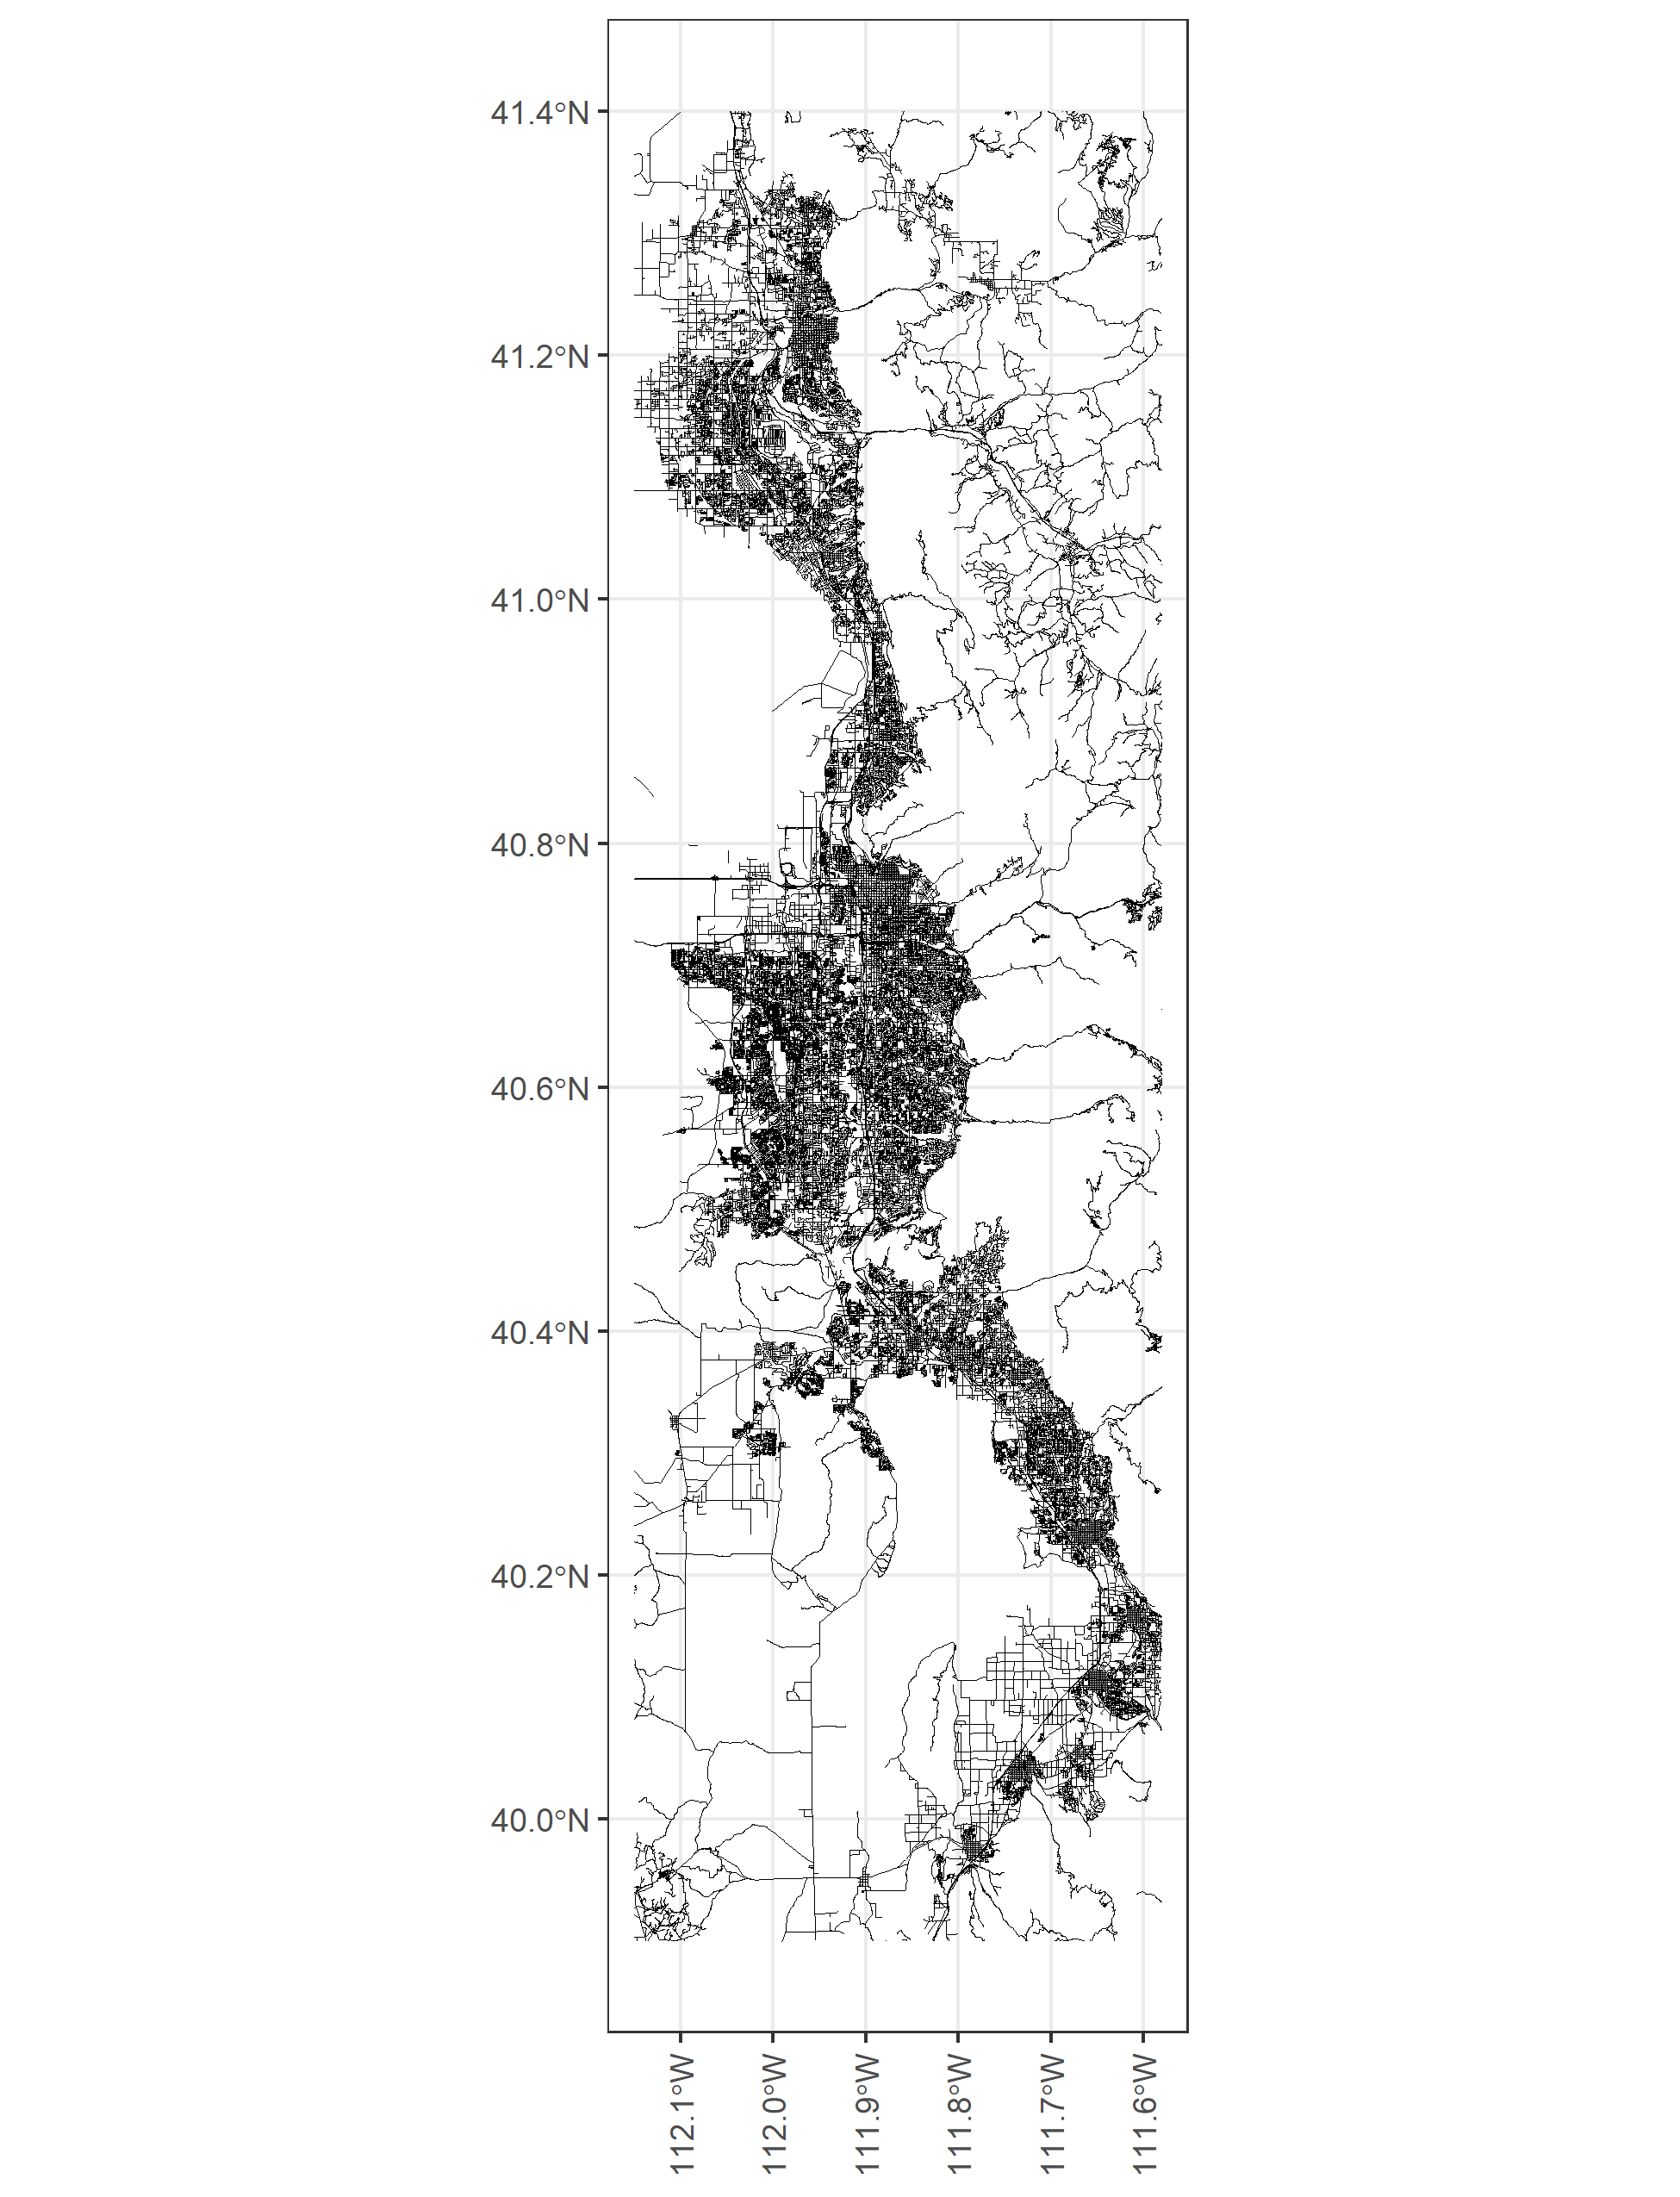
\includegraphics[width=29.17in]{pics/network} 

}

\caption{Transportation network for area of study.}\label{fig:network}
\end{figure}

\begin{figure}

{\centering 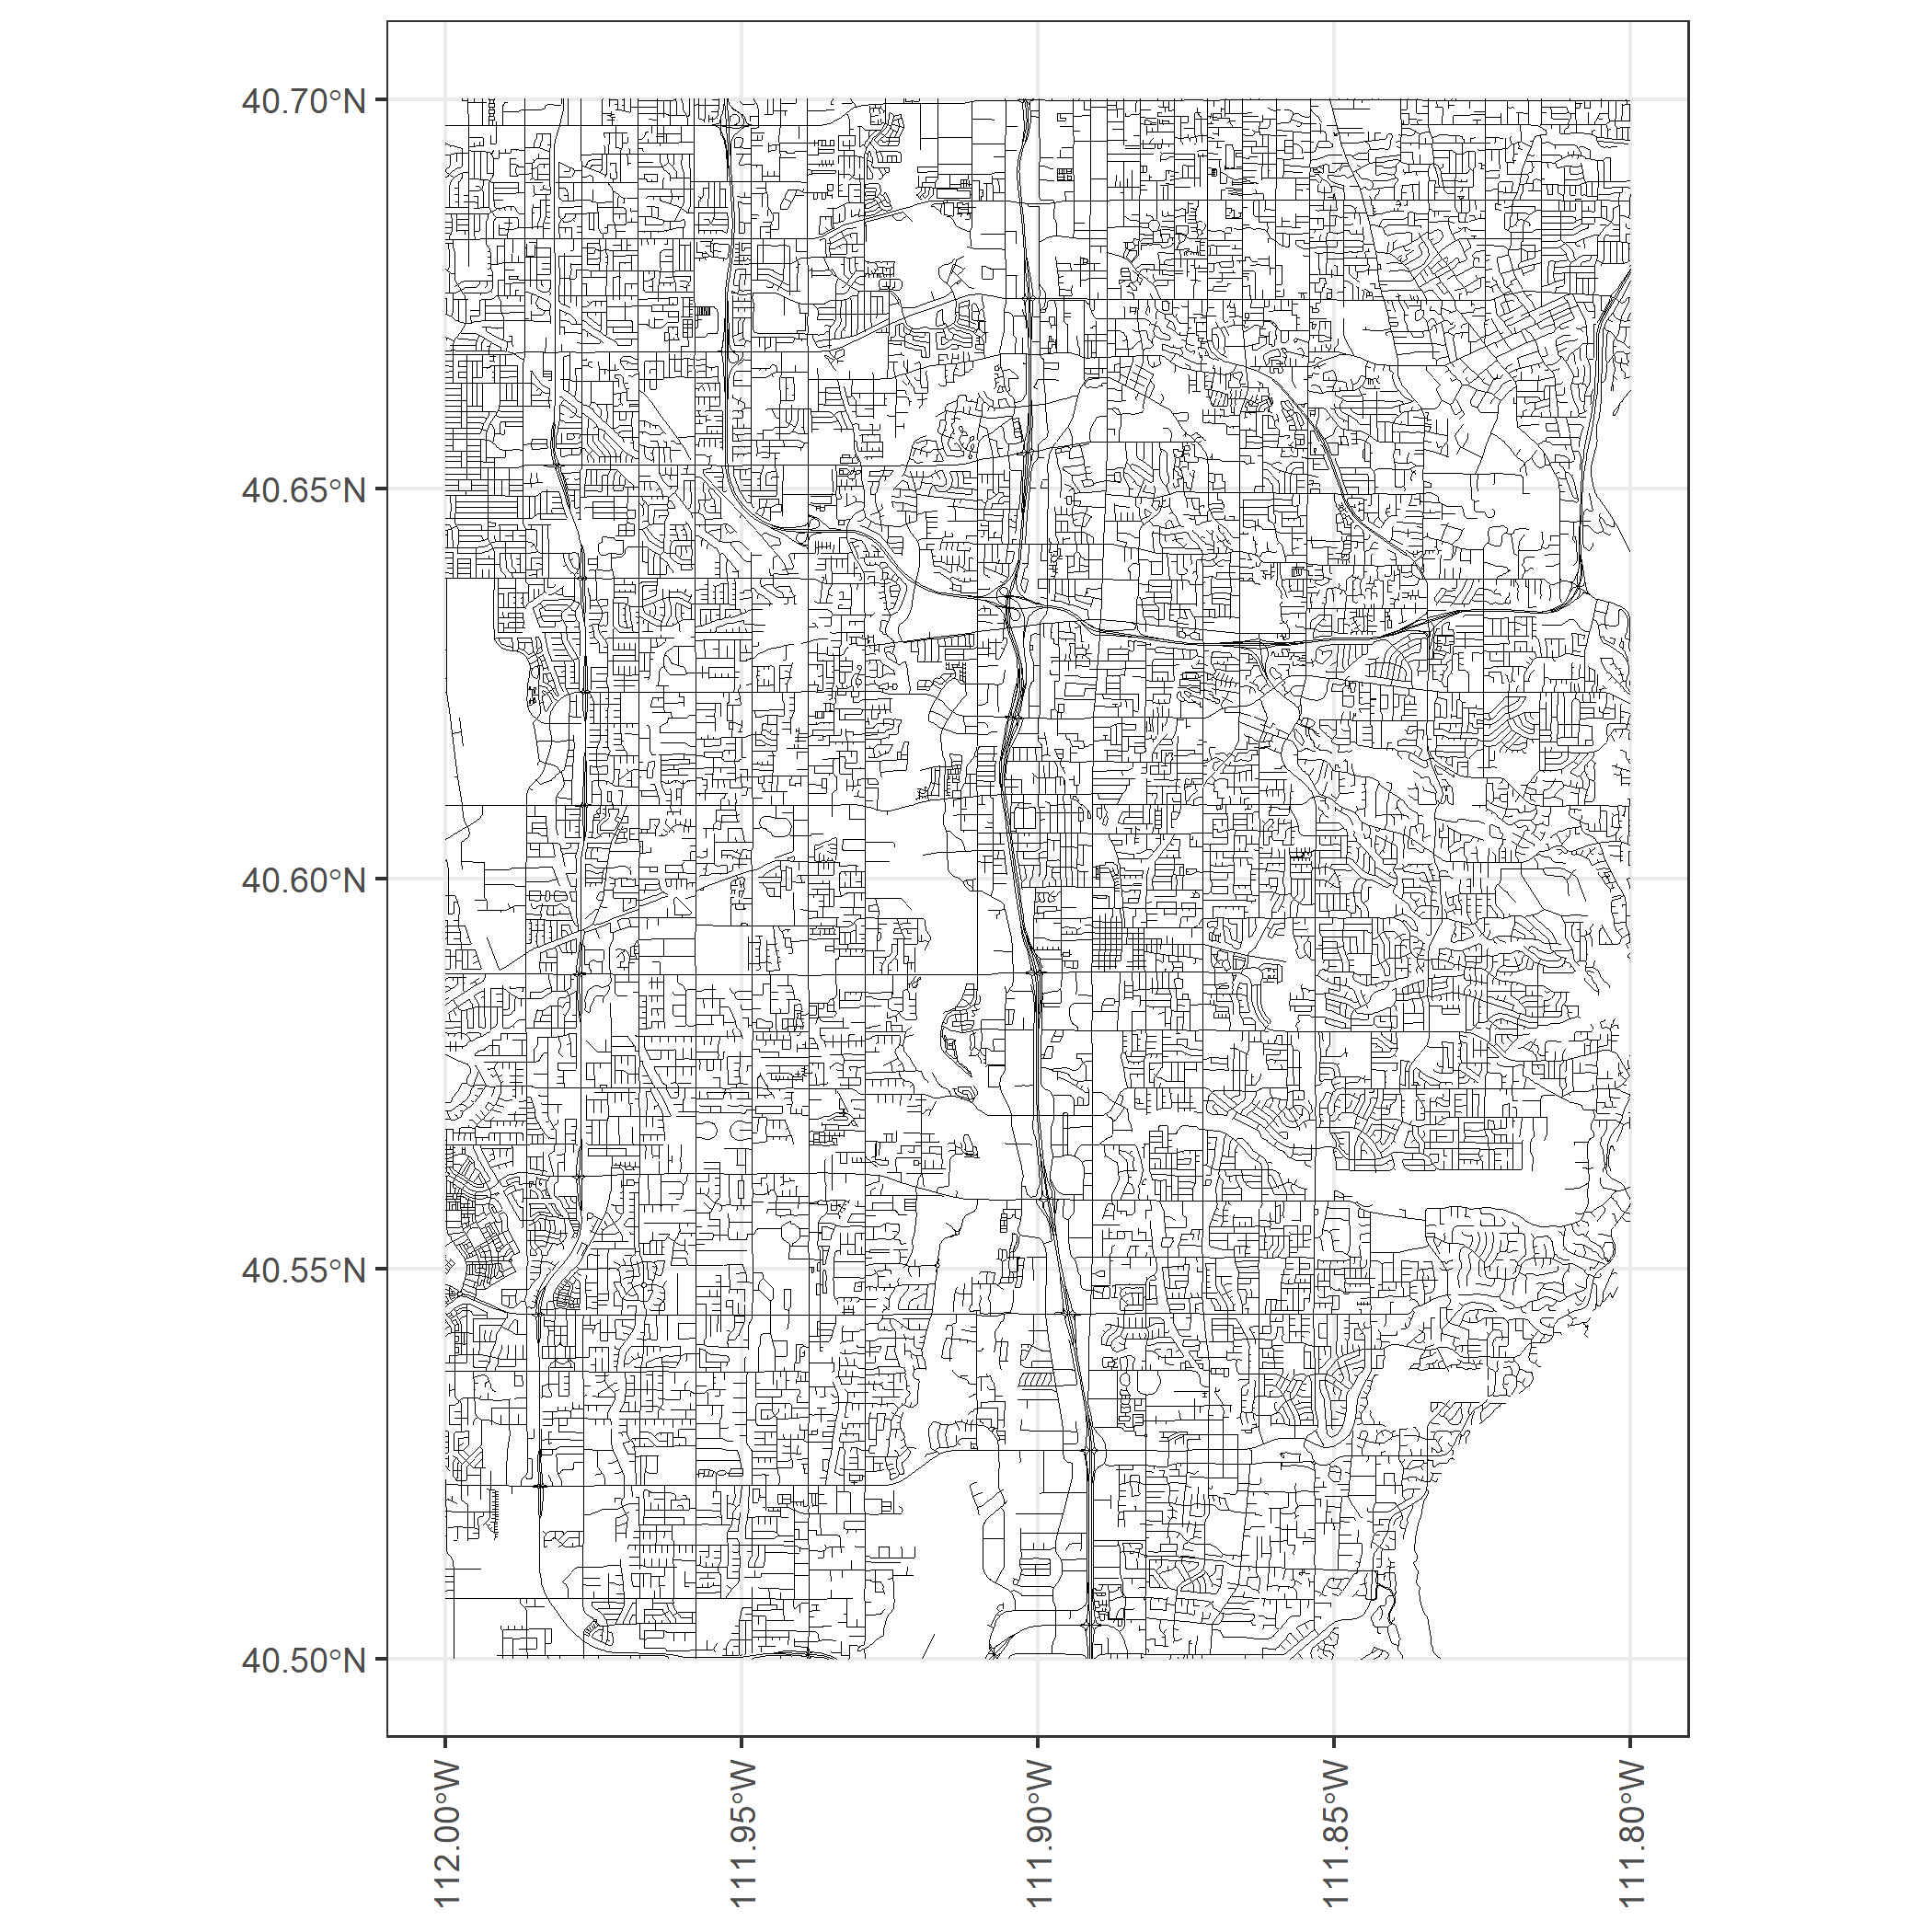
\includegraphics[width=29.17in]{pics/smallnetwork} 

}

\caption{Close up of the transportation network of Salt Lake City.}\label{fig:closent}
\end{figure}

\hypertarget{other-input-files}{%
\subsubsection{Other Input Files}\label{other-input-files}}

A variety of additional input files can be included to run the BEAM simulation. Not all the files will be mentioned, but a few of them include a configuration file, a parking file, a toll prices file, TAZ specific files, and mode choice utility parameter file. Except for the mode choice utility parameter file, details about these additional files will not be provided. The details behind the mode choice utility parameter file will be discussed in Section \ref{ute}.

\hypertarget{mbeam}{%
\section{Improved Mode Choice in BEAM}\label{mbeam}}

After creating the basic input files in order to run BEAM for the Salt Lake region, the next step was adjusting the mode choice model within BEAM itself. As discussed in Section \ref{lit7} BEAM's default mode choice model is a simple multinomial logit model calculated with minimal travel attributes. In Section \ref{lit4} it is discussed that ActivitySim's mode choice model is more comprehensive.

Changing the mode choice model within BEAM to become more consistent with that of ActivitySim's required some major adjustments to BEAM's internal code. Specifically, in this research BEAM's code was changed in three significant ways. Section \ref{purp} describes how choices were changed to be made using activity purpose values, Section \ref{ute} describes how additional attributes were inserted to the utility equation, and Section \ref{pool} describes how new modal alternatives were added to BEAM. Then, in Section\ref{algo} algorithms explaining BEAM's improved mode choice model is presented.

\hypertarget{purp}{%
\subsection{Purpose-based Decisions}\label{purp}}

The first major addition to BEAM's mode choice model to improve consistency with ActivitySim was to base mode choice decisions off of activity purposes. An activity purpose describes the primary activity of trips on a tour. Primary purposes are selected on a tour-based level. For this reason, the primary purpose is also referred to as the tour purpose. For example, if an agent were to go to the gym, then to work, and then return home, each trip on the work tour would have a primary purpose of ``work''. In this paper, tour purpose, primary purpose, activity purpose, and tour type are all used interchangeable to mean the same thing.

ActivitySim's mode choice coefficients vary between ten different tour purposes. These tour purposes are as follows:

\begin{itemize}
\tightlist
\item
  Work
\item
  University
\item
  School
\item
  Escort
\item
  Shopping
\item
  Eating Out
\item
  Social
\item
  Other Maintenance
\item
  Other Discretionary
\item
  At Work
\end{itemize}

To ensure the ability to distinguish between tour purpose values, it was necessary to adjust the population plans file to include a tour purpose trip-level attribute. Since ActivitySim bases decisions on activity purpose, it was simple to attach the attribute to the BEAM input plans file. As shown in Table \ref{tab:plans} a purpose attribute exists. After assigning this attribute to the plans, the next step was adjusting the BEAM code to read in a new attribute. By adjusting a few scripts relating to reading inputs, the primary purpose was able to be read into the BEAM software.

Once primary purpose values were present in the population plans, the next step was to design a new mode choice model within BEAM. In order to better understand the new code that was inserted into BEAM, three flow charts were constructed (See Figure \ref{fig:mnlflow}, Figure \ref{fig:lccmflow}, and Figure \ref{fig:tpcmflow}). In these flow charts inputs are displayed as folder icons, Java classes and methods are displayed as rectangles, and the result is displayed as an oval. These flow charts help display the code behind the BEAM's mode choice models. Understanding BEAM's default mode choice model and its obsolete Latent Class Choice Model (LCCM) are useful toward understanding how the new Tour Purpose Choice Model (TPCM) was constructed in the BEAM code.

\hypertarget{multinomial-logit-choice-model}{%
\subsubsection{Multinomial Logit Choice Model}\label{multinomial-logit-choice-model}}

Figure \ref{fig:mnlflow} shows the process behind BEAM's default mode choice model. As described in Section \ref{lit7}, by default BEAM calculates mode choices using a multinomial logit function with only a few attribute variables. In Figure \ref{fig:mnlflow} the flow of inputs and BEAM functions are shown. As shown, the inputs to the Mode Choice Calculator are the alternatives, person and household attributes, and the destination activity data.

\begin{figure}

{\centering 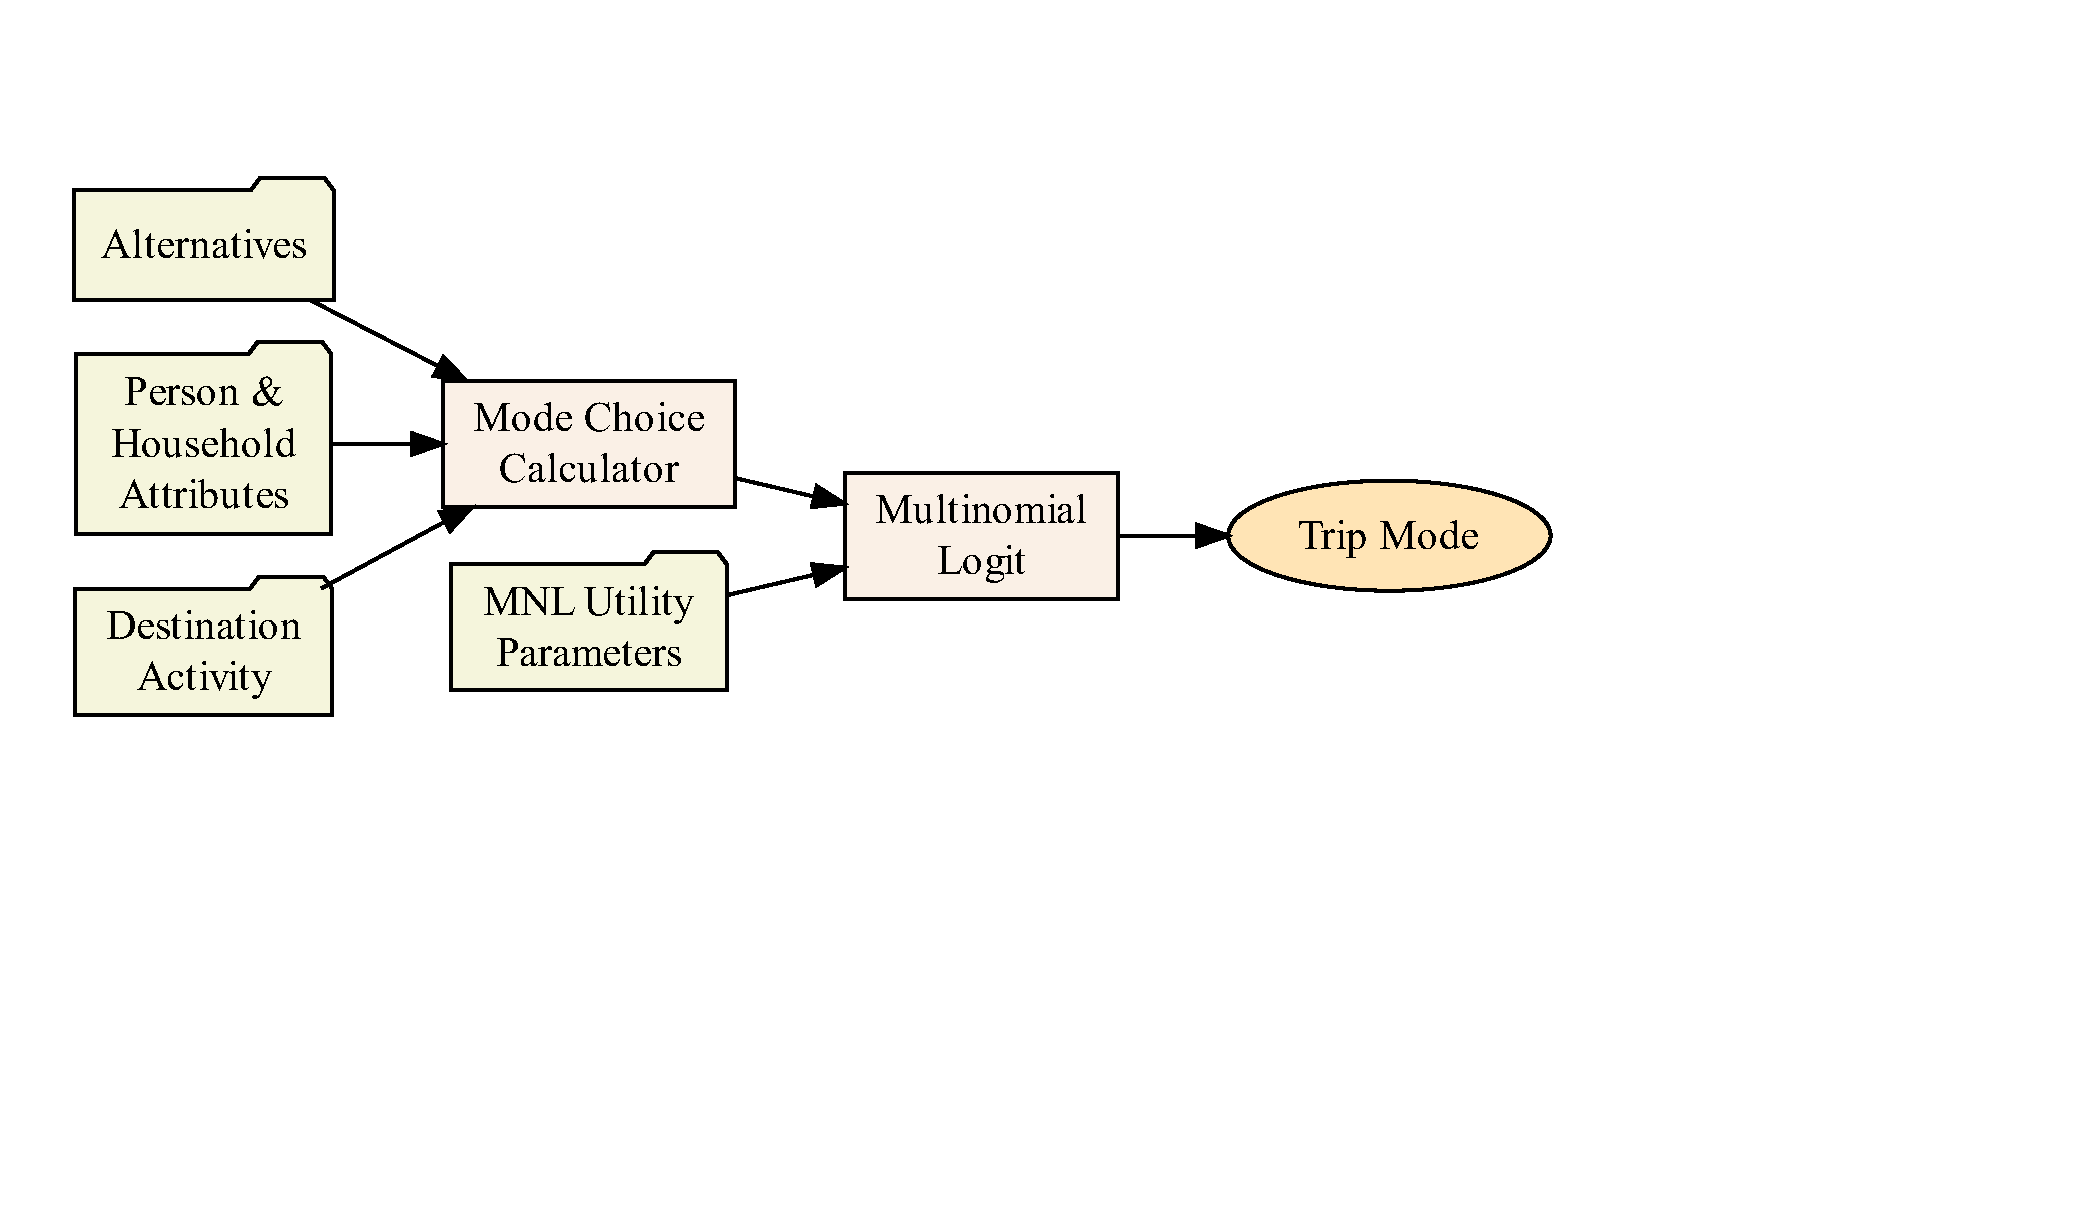
\includegraphics{thesis_files/figure-latex/mnlflow-1} 

}

\caption{BEAM code flow chart behind the default multinomial logit choice model.}\label{fig:mnlflow}
\end{figure}

The alternatives input represents a set of detailed travel itineraries that the agent can choose from. Within the alternatives variable, travel statistics, travel paths, travel modes, travel times, etc. are included. So as a result, the alternatives variable represents the modes in which the agent can choose from, while also including all the travel statistics needed to calculate the probability of selecting such mode. The next input is the person and household attributes variable. This variable includes all the information from the person attributes input file (See Table \ref{tab:peratt}) and the household attributes file (See Table \ref{tab:house}). Within the household attributes file some information from the vehicle inputs file is also included. The person and household attributes variable is also needed to calculate the probability of selecting such a mode. The last input is the destination activity data. This data simply includes additional information relating to the current trip and the destination activity. It is also useful to calculating the final mode choice.

The alternatives, person and household attributes, and destination activity are fed into the Mode Choice Calculator Java class. The purpose of this class is to organize the mode choice input data and organize it into a manner in which the choice model can process it efficiently. The Mode Choice Calculator class also houses some useful functions in the code used to calculate generalized travel time and the all day utility value.

The organized data from the Mode Choice Calculator along with the multinomial logit utility parameters are then sent to the multinomial logit choice model. The utility parameters in the default BEAM code are simply expressed in the configuration file. For each mode, an intercept, transit occupancy level, and transfer intercept/multiplier is specified. Then, within the multinomial logit choice model the utility value is calculated for each modal alternative. Those utility values are then sampled and one final mode is chosen!

\hypertarget{latent-class-choice-model}{%
\subsubsection{Latent Class Choice Model}\label{latent-class-choice-model}}

BEAM has an obsolete LCCM within its code structure. When BEAM was first being developed, the LCCM was how modal decisions were made. Part of creating the new Tour Purpose Choice Model was first to recreate and reboot the LCCM and second to change its structure slightly to base decisions off of tour purpose. For this reason, the structure behind the LCCM is presented. Figure \ref{fig:lccmflow} shows the flow of code for the LCCM.

\begin{figure}

{\centering 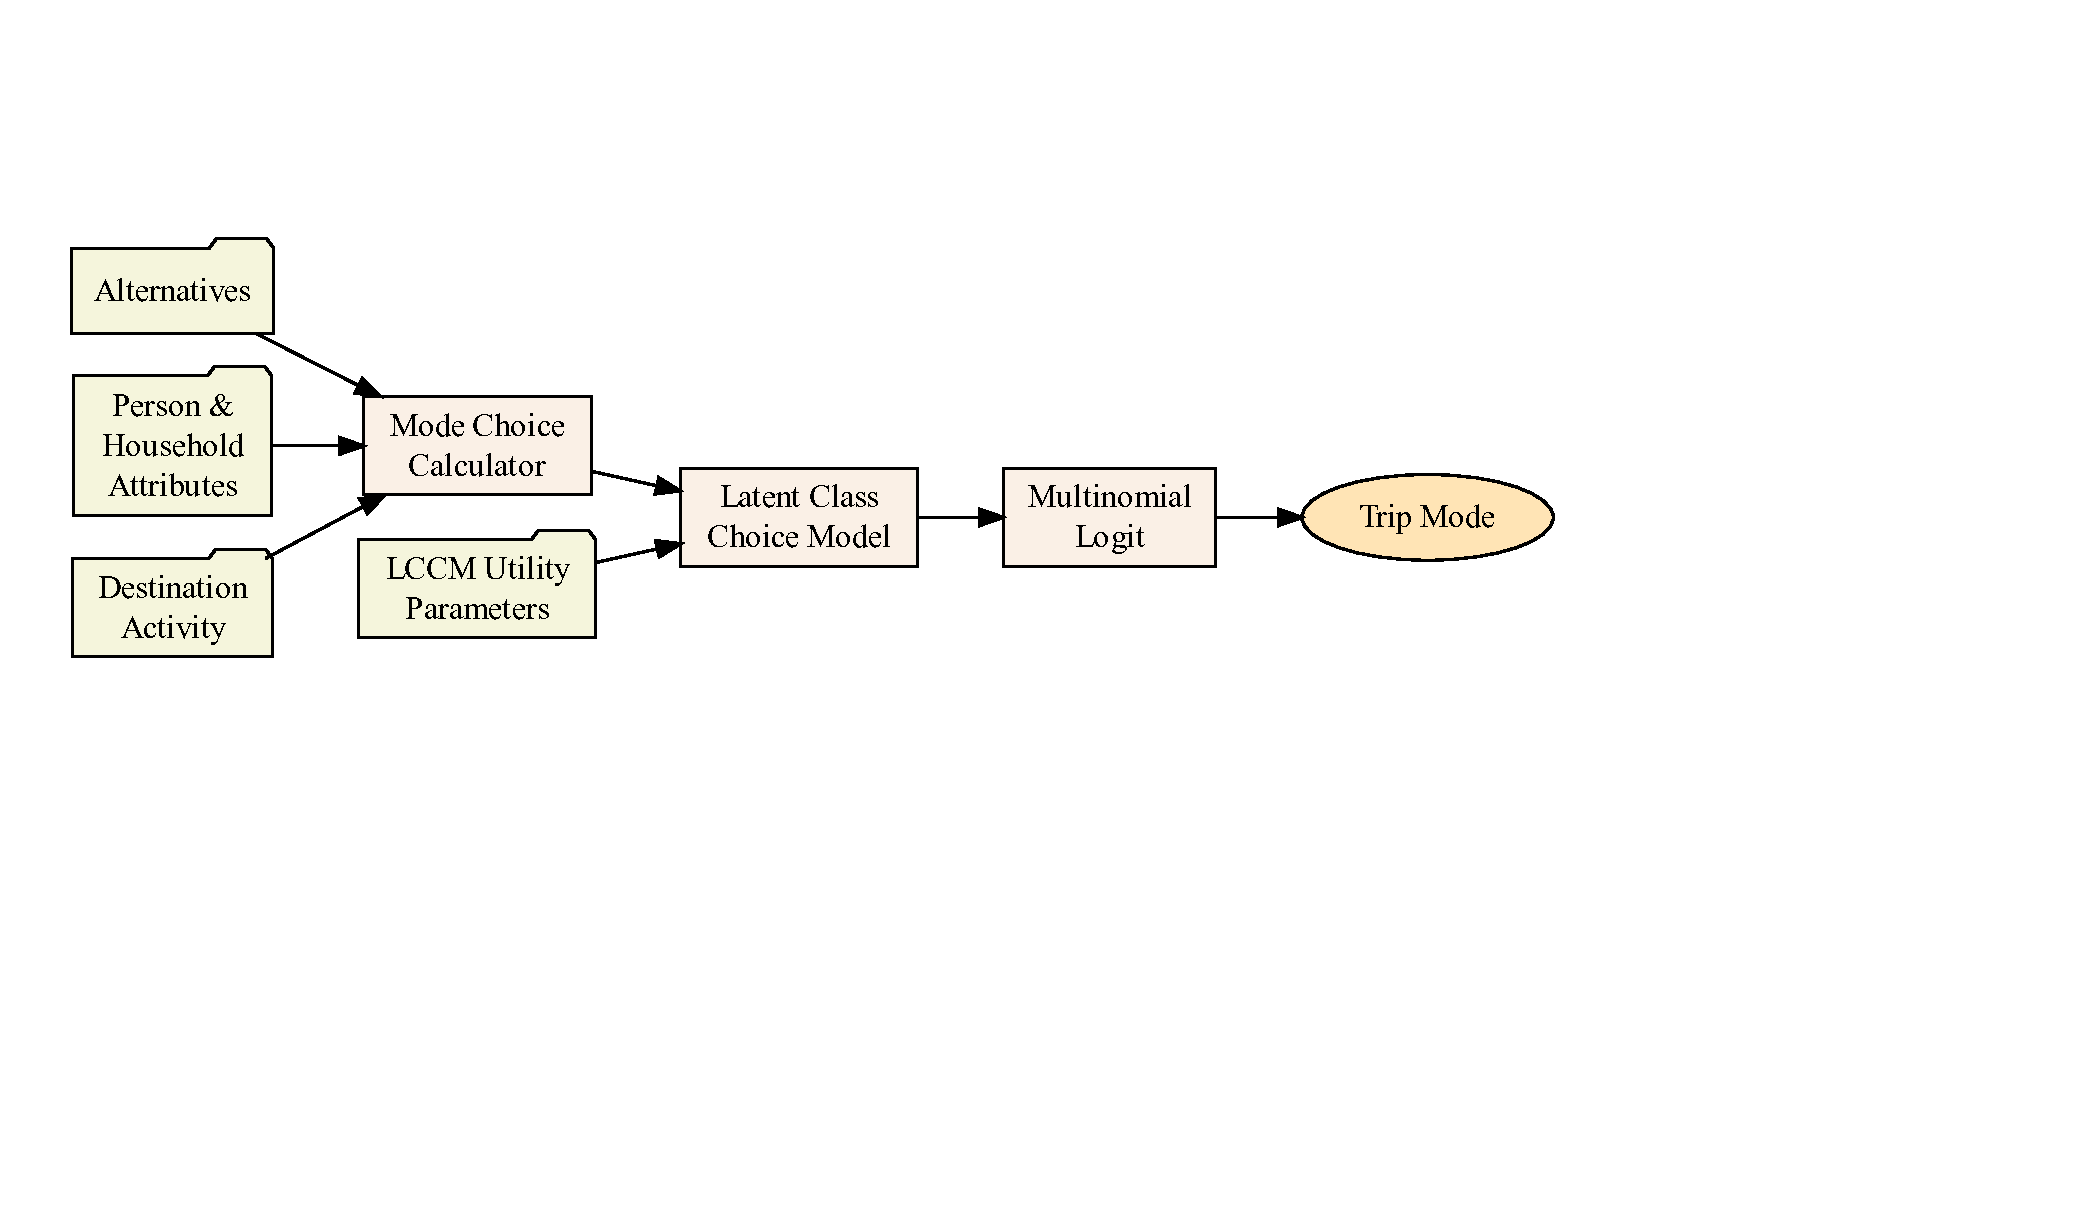
\includegraphics{thesis_files/figure-latex/lccmflow-1} 

}

\caption{BEAM code flow chart behind the latent class choice model.}\label{fig:lccmflow}
\end{figure}

Just like with the multinomial logit choice model, the same alternatives, person and household attributes, and destination activity inputs are fed into the Mode Choice Calculator. The Mode Choice Calculator then acts in a similar way to organize the data for further analysis. However, an additional step is taken where the information is sent to a Latent Class Choice Model Java class before it is sent to the Multinomial Logit Java class. Within the Latent Class Choice Model Java class, a few things happen. First, the LCCM Utility Parameters data file is read into the code and parsed. After parsing the data, the utility parameters are attached to each alternative and stored.

The LCCM Utility Parameters file includes mode choice coefficients relating to number of cars, household size, income, cost, time, and also alternative specific constants. The interesting part to the LCCM is that it calculates modes based off of which \emph{modality style} a particular agent is a part of. The \emph{modality style} represents the travel behavior of the individual. The LCCM code divides individuals up into one of the six groups or classes based on their \emph{modality style} travel behavior. The LCCM BEAM code provides two incredibly useful structures that are directly related to creating the TPCM. First, it provides a code structure that reads in a file storing specific and attribute related utility parameters. Second, it provides a code structure for storing these utility parameters into each alternative based on person/household attributes, travel statistics, and destination activity.

Interestingly enough, after the Latent Class Choice Model Java class reads in the utility information and stores it accordingly, it is sent to the same Multinomial Logit Java class. The overall utility value is calculated for each alternative and then are sampled down to a final mode choice!

\hypertarget{tour-purpose-choice-model}{%
\subsubsection{Tour Purpose Choice Model}\label{tour-purpose-choice-model}}

As mentioned previously, the TPCM was constructed off of the LCCM within BEAM. This means the first step to creating this model was fixing the LCCM and making the LCCM run correctly. With a few minimal code adjustments, and a lot of debugging, the LCCM was brought back to life. The final flow of code for the TPCM is presented in Figure \ref{fig:tpcmflow}.

\begin{figure}

{\centering 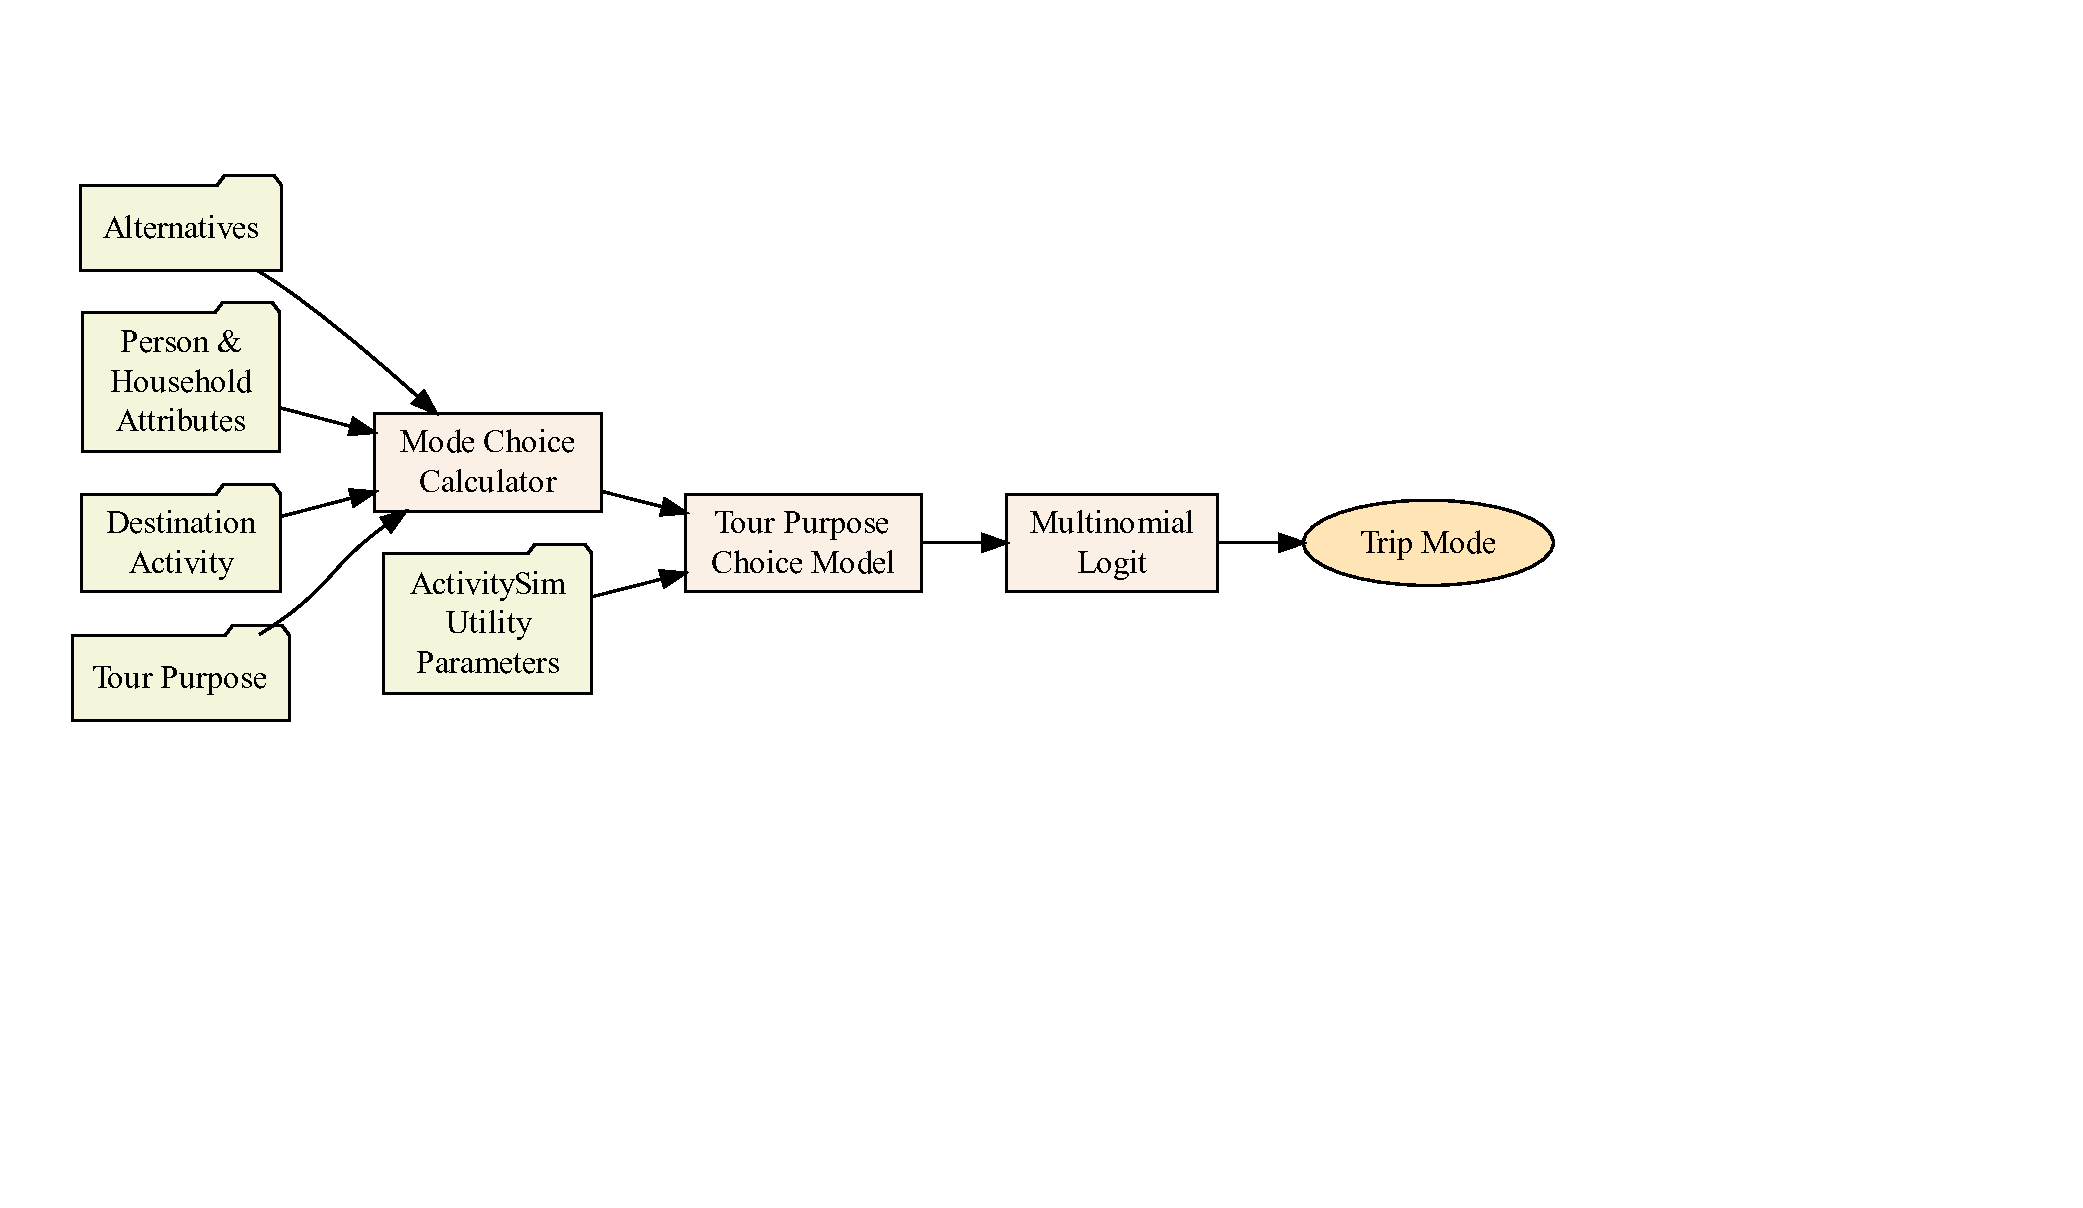
\includegraphics{thesis_files/figure-latex/tpcmflow-1} 

}

\caption{BEAM code flow chart behind the tour purpose choice model.}\label{fig:tpcmflow}
\end{figure}

The flow chart shows a very similar choice process as the LCCM, except that an additional input is sent to the Mode Choice Calculator. Obviously, the tour purpose value is necessary for the choice model and is therefore also sent to the Mode Choice Calculator. This input is only available, however, because it was attached to the population plans as explained previously.

In order to create the TPCM, two main steps were taken. First, a Tour Purpose Choice Model Java class was developed, mimicking how the code worked within the Latent Class Choice Model Java class. The TPCM was much more advanced than the LCCM, however, because instead of six classes to choose from there were ten activity purposes to choose from. In addition, instead of only needing a few travel statistics to do the mode choice, the TPCM included 25 different path, person, and location type variables. The second step toward creating the TPCM was to develop an input csv file that included all the utility parameter values from ActivitySim. These additional attributes used in the utility equation are discussed in Section \ref{ute}.

Overall, the Tour Purpose Choice Model Java class performed similarly to the Latent Class Choice Model Java class. It was able to parse the input utility parameters, attach those values to the alternatives, as well as calculate the travel statistics for all 25 travel variables. To do this, an additional class was built to calculate each of the travel variables. The final mode choice was determined in the same manner as well. These alternatives were sent to the Multinomial Logit Java class where their modal utilities were calculated and sampled. The sampling then determined a final mode choice for each individual.

\hypertarget{ute}{%
\subsection{Additional Attributes in Utility Equation}\label{ute}}

Equally important to developing the tour purpose choice model code structure within BEAM was to develop a consistent mode choice utility function. As explained in Section \ref{lit4} ActivitySim bases its mode choice off of an abundance of path, person, and location type variables. Therefore, most of these path, person, and location type variables were inserted into the BEAM structure and used to calculate mode choice. The travel statistics for each variable were calculated within the TPCM code and the coefficient and intercept parameter values were included using an input file.

The input file for the utility calculation included every combination of variable, mode, and purpose. For example, what is the cost coefficient for a drive transit trip on a school tour? With 25 different variables, 11 different modes, and 10 different tour purposes, a total of 3251 parameter values existed! Of course, a large portion of these combinations were left blank. (For example, the walk distance variable was only applied to walk type modes.) These parameter values were obtained from a variety of sources.

The alternate specific constants were obtained from the utility values used in the example\_mtc scenario from the ActivitySim software (ActivitySim 2021). These constants were used in the initial stages of modeling, but were then updated and calibrated to the Salt Lake Region in Section \ref{clib}. The majority of the coefficient values were obtained from the tour mode choice coefficients from MTC (2012). Since BEAM's mode choice is trip-based however, all these tour-based coefficients were multiplied by two and then used as trip-based coefficients. The trip-based coefficients from MTC (2012) were not used because they did not provide the same level of precision and thoroughness as the tour-based coefficients. Tour values were hence doubled as to better represent trip characteristics. In places where coefficients and constants did not exist for certain modes, the values of its most similar mode were used instead, sometimes with slight adjustments. For example, the bike transit constants did not exist so the walk transit values were used instead of leaving its values empty. Below, a list of the path, person, and location variables used to calculate the modal utility is shown. Not all 25 variables are listed since some of the variables describe a group of variables.

\begin{itemize}
\tightlist
\item
  \emph{Path Variables}: Number of Transfers, Vehicle Time, Egress Time, Wait Time, Origin to Transit Proximity, Destination to Transit Proximity, Walking Distance, Biking Distance, and Driving Distance
\item
  \emph{Person Variables}: Cost, Age, Household Size, and Vehicle to Worker Ratio
\item
  \emph{Location Variables}: Zonal Destination Index and Central Business District
\end{itemize}

In addition, Table \ref{tab:asimvals} shows a subsection of the input file with only the cost variable coefficients provided. The purpose of showing this table is to help understand how extensive the choice model was. Within the table it is clear to see that variation exists between tour purpose, modal alternative, and variable type. Only three modal alternatives are provided in the table.

\begin{table}

\caption{\label{tab:asimvals}Cost coefficient values for some modes from the utility parameters csv file}
\centering
\begin{tabular}[t]{lllllr}
\toprule
Variable Type & Variable & Alternative & Units & Tour Purpose & Value\\
\midrule
Person & cost & car & util/min & work & -0.026\\
Person & cost & car & util/min & univ & -0.044\\
Person & cost & car & util/min & school & -0.044\\
Person & cost & car & util/min & escort & -0.036\\
Person & cost & car & util/min & shopping & -0.036\\
\addlinespace
Person & cost & car & util/min & eatout & -0.036\\
Person & cost & car & util/min & othmaint & -0.036\\
Person & cost & car & util/min & social & -0.036\\
Person & cost & car & util/min & othdiscr & -0.036\\
Person & cost & car & util/min & atwork & -0.038\\
\addlinespace
Person & cost & ride\_hail & util/min & work & -0.026\\
Person & cost & ride\_hail & util/min & univ & -0.044\\
Person & cost & ride\_hail & util/min & school & -0.044\\
Person & cost & ride\_hail & util/min & escort & -0.036\\
Person & cost & ride\_hail & util/min & shopping & -0.036\\
\addlinespace
Person & cost & ride\_hail & util/min & eatout & -0.036\\
Person & cost & ride\_hail & util/min & othmaint & -0.036\\
Person & cost & ride\_hail & util/min & social & -0.036\\
Person & cost & ride\_hail & util/min & othdiscr & -0.036\\
Person & cost & ride\_hail & util/min & atwork & -0.038\\
\addlinespace
Person & cost & walk\_transit & util/min & work & -0.026\\
Person & cost & walk\_transit & util/min & univ & -0.044\\
Person & cost & walk\_transit & util/min & school & -0.044\\
Person & cost & walk\_transit & util/min & escort & -0.036\\
Person & cost & walk\_transit & util/min & shopping & -0.036\\
\addlinespace
Person & cost & walk\_transit & util/min & eatout & -0.036\\
Person & cost & walk\_transit & util/min & othmaint & -0.036\\
Person & cost & walk\_transit & util/min & social & -0.036\\
Person & cost & walk\_transit & util/min & othdiscr & -0.036\\
Person & cost & walk\_transit & util/min & atwork & -0.038\\
\bottomrule
\end{tabular}
\end{table}

The observable utility equation for the new tour purpose choice model can be divided up into three sub-equations. Equation \eqref{eq:tpcmpath} shows the Path type variable part of the TPCM utility equation. Equation \eqref{eq:tpcmperson} shows the Person type variable part of the TPCM utility equation. Equation \eqref{eq:tpcmloc} shows the Location type variable part of the the TPCM utility equation. The full TPCM utility equation, however, is the combination of path, person, and location type variables, as displayed in Equation \eqref{eq:tpcmall}.

\hypertarget{path-type-utility-equation}{%
\subsubsection{Path Type Utility Equation}\label{path-type-utility-equation}}

\begin{equation}
  V_j = \beta_{t_v}(t_v) + \beta_{t_w}(t_w) + \beta_{t_e}(t_e) + \beta_{tr_p}(tr_p) + \beta_{xfer}(xfer) + \beta_{w_{dis}}(w_{dis}) + \\ \beta_{b_{dis}}(b_{dis}) + \beta_{d_{dis}}(d_{dis}) \label{eq:tpcmpath}
\end{equation}

where

\begin{itemize}
\tightlist
\item
  \(j\) is the modal alternative,
\item
  \(t_v\) is the in vehicle travel time (mins),
\item
  \(t_w\) is the wait time (mins),
\item
  \(t_e\) is the egress time (mins),
\item
  \(tr_p\) is the proximity to transit (miles),
\item
  \(xfer\) is the number of transfers,
\item
  \(w_{dis}\) is the walk distance (miles),
\item
  \(b_{dis}\) is the bike distance (miles),
\item
  \(d_{dis}\) is the drive distance (miles),
\item
  \(\beta_{tr_p}\) differs between origin/destination and length, and
\item
  \(\beta_{w_{dis}}\), \(\beta_{b_{dis}}\), and \(\beta_{d_{dis}}\) differ between lengths.
\item
  \emph{Note:} All \(\beta\) values differ between mode and tour purpose.
\end{itemize}

\hypertarget{person-type-utility-equation}{%
\subsubsection{Person Type Utility Equation}\label{person-type-utility-equation}}

\begin{equation}
  V_j = ASC_{auto} +  \beta_{c}(c) + \beta_{ag}(ag) \label{eq:tpcmperson}
\end{equation}

where

\begin{itemize}
\tightlist
\item
  \(j\) is the modal alternative,
\item
  \(ASC_{auto}\) is the alternative specific constant that differs between modal alternative and auto ownership dependency,
\item
  \(c\) is the cost, and
\item
  \(ag\) is the age grouping (if the person is between 0-10 or 16-19 years old).
\item
  \emph{Note:} All \(\beta\) values differ between mode and tour purpose.
\end{itemize}

\hypertarget{location-type-utility-equation}{%
\subsubsection{Location Type Utility Equation}\label{location-type-utility-equation}}

\begin{equation}
  V_j = \beta_{zdi}(zdi) + \beta_{cbd}(cbd) \label{eq:tpcmloc}
\end{equation}

where

\begin{itemize}
\tightlist
\item
  \(j\) is the modal alternative
\item
  \(zdi\) is the zonal density index,
\item
  \(cbd\) is a classifier for zones labeled as central business district, and
\item
  \(\beta_{zdi}\) differs between origin/destination.
\item
  \emph{Note:} All \(\beta\) values differ between mode and tour purpose.
\end{itemize}

\hypertarget{beams-new-consistent-utility-equation}{%
\subsubsection{BEAM's New Consistent Utility Equation}\label{beams-new-consistent-utility-equation}}

\begin{equation}  
  V_j = Eq:4.1 + Eq:4.2 + Eq:4.3 \label{eq:tpcmall}
\end{equation}

where

\begin{itemize}
\tightlist
\item
  \(j\) is the modal alternative.
\end{itemize}

When comparing Equation \eqref{eq:tpcmall} with BEAM's default equation in Equation \eqref{eq:beammnl}, it is clear that multiple more travel variables are used to calculate the utility value. When comparing this Equation \eqref{eq:tpcmall} with the ActivitySim equations in Section \ref{lit4}, most of the same variable are used. By using most of the path, person, and location type variables to calculate the mode choice, the TPCM calculates utility in a consistent manner with ActivitySim. In addition, all utility values differ by tour purpose, making it almost identical to ActivitySim's trip-based mode choice.

It is important to note that BEAM's internal code is built on a trip-based level, and so no overarching tour mode choice was determined before trip mode choice. It was outside the scope of this project to adjust BEAM's structure to include a tour mode choice model. As a result, the mode choice consistency only exists on the trip-based mode choice level. Hopefully, in the future a consistent tour-based mode choice can be inserted into BEAM as well.

\hypertarget{pool}{%
\subsection{Carpool Alternatives}\label{pool}}

After designing a tour purpose choice model within BEAM and extending the mode choice utility equation, more consistency with ActivitySim was achieved by adding additional modal alternatives. BEAM by default includes nine modal alternatives. ActivitySim, however has eight upper level mode choices and 18 total mode choices. The lower level mode choices include distinctions between car and carpool modes being paid or not, and five different types of transit modes. For simplicity, BEAM's modes will be compared to ActivitySims upper level mode choice categories. Figure \ref{fig:venn} shows a venn diagram of how the modes compare between BEAM and ActivitySim.

\begin{figure}

{\centering 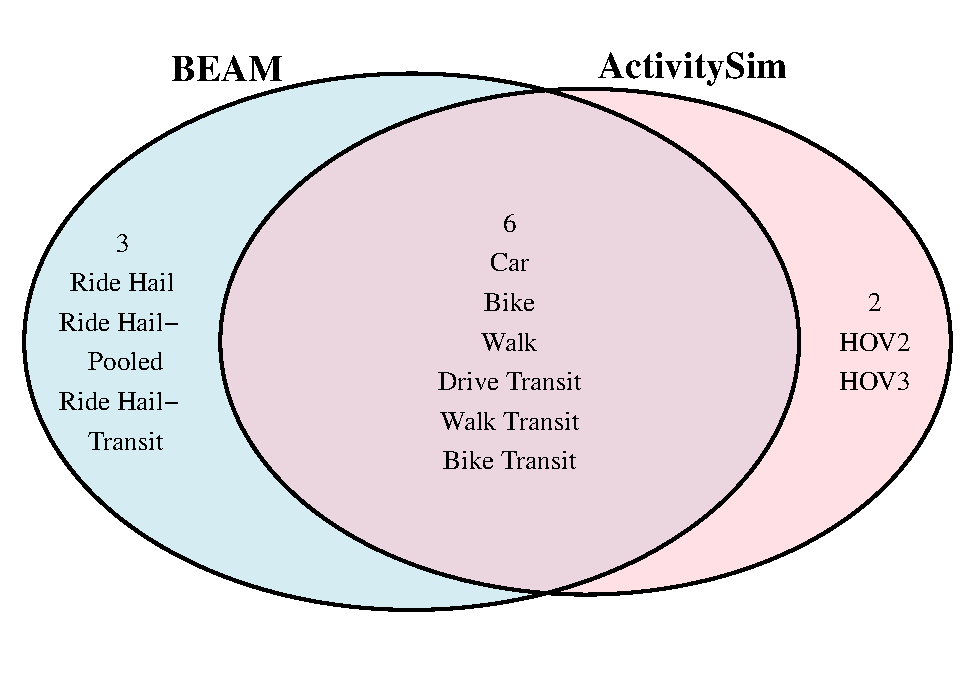
\includegraphics{thesis_files/figure-latex/venn-1} 

}

\caption{A comparison between BEAM and ActivitySim's modal alternatives.}\label{fig:venn}
\end{figure}

As seen in Figure \ref{fig:venn}, both BEAM and ActivitySim include car, bike, walk, and various types of transit modes. BEAM includes ride hailing modal alternatives whereas ActivitySim includes carpooling alternatives (HOV2 and HOV3). HOV2 means High Occupancy Vehicle with 1 passenger (2 people in the vehicle) and HOV3 means High Occupancy Vehicle with 2 or more passengers (at least 3 people in the vehicle). Both HOV2 and HOV3 simply represent the option to carpool. Therefore, to create more consistency with ActivitySim, carpooling/HOV alternatives were added into the BEAM mode choice model.

Four new carpooling alternatives were added to BEAM: HOV2, HOV2\_TELEPORTATION, HOV3, and HOV3\_TELEPORTATION. HOV2 and HOV3 were coded to act identical to car modes. They were mapped to the network and thus could add to congestion. Their travel statistics were also calculated in the same way as for car modes. Agents who selected HOV2 or HOV3 were represented as the drivers of the carpooling cars. HOV2\_TELEPORTATION and HOV3\_TELEPORTATION modes were added to the modal alternative options as to represent non driving carpooling agents / passengers. These agents would simply teleport to their destination as to not add extra congestion to the network. Their travel statistics, however, were still calculated to represent a car traveling from the origin to the destination. Adding both car and teleporting HOV modes allowed carpooling alternatives to be represented as accurately as possible within the BEAM code.

Within the code, HOV2 and HOV3 modes were provided as modal options by transforming an existing car option into an HOV option. By doing this, HOV modes did not have to be added to the R5 routing engine (Conveyal 2022). The R5 routing engine helps BEAM accomplish multi-modal routing. For the default modes with BEAM, agents make a request to the router and then the routing system calculates a distinct route through the system for all possible modal options (BEAM 2022). Car alternatives from the router were copied and changed into HOV2 and HOV3 options for agents to choose from. This allows car travel statistics to be transferred over to the carpooling modes.

In cases where car routes were not provided from the router, HOV2 and HOV3 options could not be created. Often times this occurred for agents that did not have access to a car. This birthed the question of how to provide carpooling vehicles to agents without their own vehicle? In the real world, plenty of people without vehicles get rides from their friends. Therefore, as a way to surpass this problem, teleportation HOV vehicles were provided to these agents. In these cases, walk routes from the router were transformed into teleportation routes. Car travel statistics like travel time were calculated using the input skim data. In addition, costs for all teleportation modes were set to \$0, as oftentimes in the real world when picking up a friend that friend does not contribute to drive costs. Overall, by transforming existing routes from the router into carpooling alternatives, the ability to carpool became possible within BEAM. The carpooling addition thus made BEAM more consistent with the ActivitySim mode choice model.

\hypertarget{algo}{%
\subsection{Mode Choice Algorithms}\label{algo}}

As a way to better understand the complexity behind the code changes within BEAM, two pseudocode algorithms are provided. Specifically, the algorithms are meant to provide clarification on how BEAM's new mode choice model works.

Algorithm 1 describes the process behind determining the mode choice alternatives for each agent. This process occurs for every agent for every trip. Two procedures are presented within the first algorithm. The first procedure is called DetermineHOVAlternatives. This procedure was added to the BEAM code as a way to include carpooling options. In this procedure the process explained in Section \ref{pool} is shown where HOV alternatives are created from already existing options created by the router. Basically if a car, HOV2, or HOV3 mode is already created from the router, then both HOV2 and HOV3 options are provided. If car is not provided by the router, then teleporting HOV options are provided. The second procedure within Algorithm 1 describes the process behind determining the final modal alternatives. It essential states that if the current mode is already chosen, then that mode remains as the only alternative to choose from. However, if no mode is currently chosen for the trip, the router, ride hailing, and HOV alternatives are combined and presented as the final alternatives to choose from.

\begin{algorithm} [tph]
\caption{Algorithm for Determining Mode Choice Alternatives in BEAM}
\begin{algorithmic}[1]
\Require
\State $i : origin$
\State $j : destination$
\State $n: agent$
\State $N: population$
\State $t : trip $
\State $P : plan$
\State $\vec{R}(i,j) : Router\: alternatives$
\State $\vec{RH}(i,j) : Ridehail\:alternatives$
\State $\vec{H}(i,j) : HOV\:alternatives$
\State $\vec{M}(i,j) : Final\:modal\:alternatives$
\State $C : Current\:Mode$
\State $I : Trip\:Index$
\vspace{4pt}\hrule\vspace{5pt}

\State $\vec{R} \equiv \vec{R}(i,j)$
\State $\vec{RH} \equiv \vec{RH}(i,j)$
\State $\vec{H} \equiv \vec{H}(i,j)$
\State $\vec{M} \equiv \vec{M}(i,j)$
\For {$n \in N$}
\For {$t \in P$}

\Procedure {DetermineHOVAlternatives}{$\vec{R}$, $C$}
\If {$C=None$}
  \If {$\vec{R} \ni CAR$}
    \State $\vec{H} \gets (HOV2,HOV3)$
  \ElsIf {$\vec{R} \ni HOV2$}
    \State $\vec{H} \gets (HOV3)$
  \ElsIf {$\vec{R} \ni HOV3$}
    \State $\vec{H} \gets (HOV2)$
  \ElsIf {$\vec{R} \ni WALK$}
    \State $\vec{H} \gets (HOV2\_TELEPORT, HOV3\_TELEPORT)$
  \EndIf
\Else
  \State $\vec{H} \gets None$
\EndIf
\EndProcedure
\Statex
\algstore{myalg}
\end{algorithmic}
\end{algorithm}

\addtocounter{algorithm}{-1}
\begin{algorithm}
\caption{continued}
\begin{algorithmic} [1]
\algrestore{myalg}
\Procedure {DetermineFinalModalAlternatives}{$\vec{R}$, $\vec{RH}$, $\vec{H}$, $C$, $I$}
\If {$C = DRIVE\_TRANSIT \lor BIKE\_TRANSIT$}
  \If {$I = 0$}
    \If {$C = DRIVE\_TRANSIT$}
      \State $\vec{M} \gets (DRIVE\_TRANSIT)$
    \Else
      \State $\vec{M} \gets (BIKE\_TRANSIT)$
    \EndIf  
  \Else
    \State $\vec{M} \gets (WALK\_TRANSIT, RIDEHAIL\_TRANSIT)$
  \EndIf
\ElsIf {$C = WALK\_TRANSIT \lor RIDEHAIL\_TRANSIT$}  
  \If {$C = WALK\_TRANSIT$}
    \State $\vec{M} \gets (WALK\_TRANSIT)$
  \Else
    \State $\vec{M} \gets (RIDEHAIL\_TRANSIT)$
  \EndIf
\ElsIf {$C = HOV2\_TELEPORT \lor HOV3\_TELEPORT$}  
  \If {$C = HOV2\_TELEPORT$}
    \State $\vec{M} \gets (HOV2\_TELEPORT)$
  \Else
    \State $\vec{M} \gets (HOV3\_TELEPORT)$
  \EndIf
\ElsIf {$C = CAR$}
  \State $\vec{M} \gets (CAR)$
\Else
  \State $\vec{M} \gets \vec{R} + \vec{RH} + \vec{H}$  
\EndIf  
\EndProcedure
\EndFor
\EndFor
\Statex
\end{algorithmic}
\end{algorithm}

Algorithm 2 describes the process within BEAM for how one modal alternative is selected among all the mode choice options. Algorithm 2 is basically the pseudocode behind the process that occurs within the Multinomial Logit Java class presented in Figure \ref{fig:mnlflow}, Figure \ref{fig:lccmflow}, and Figure \ref{fig:tpcmflow}. Within this class, as shown in Algorithm 2, the math behind the mulitnomial logit formula is shown. Then, after using the multinomial logit formula, the probabilities that were calculated are sampled and one final mode choice alternative is selected!

\begin{algorithm}
\caption{Algorithm for Selecting Final Modal Alternative in BEAM}
\begin{algorithmic}[1]
\Require
\State $i : origin$
\State $j : destination$
\State $n: agent$
\State $N: population$
\State $t : trip $
\State $P : plan$
\State $\vec{A}: attributes\:of\:agent$
\State $a: attribute\:value$
\State $\vec{M}(i,j) : Modal\:alternatives$
\State $m : alternative \in M(i,j)$
\State $\vec{U}(\vec{M}(i,j),\vec{A}):Utilities\:for\:alternatives$
\State $u: utility \in \vec{U}(\vec{M}(i,j),\vec{A})$
\State $\vec{c}: attribute\:coefficients$
\State $\mathds{P}: probability$
\State $Mode: chosen\:mode\:for\:agent\:(n)\:on\:trip\:(t)$
\State $f(\vec{X}):$
This function takes a vector of modes and  their probabilities of being chosen. With those probabilities it builds them into a cumulative distribution function, generates a random number and then drops the mode with the closest probability. This process continues until only one mode is left.
\vspace{4pt}\hrule\vspace{5pt}

\State $\vec{M} \equiv \vec{M}(i,j)$
\State $\vec{U} \equiv \vec{U}(\vec{M},\vec{A})$
\For {$n \in N$}
\For {$t \in P$}\Procedure {DetermineFinalModalAlternative}{$\vec{M}$, $\vec{A}$, $\vec{c}$}
\For {$m \in \vec{M}$}
  \State $u \gets \sum_{a\in \vec{A}} a \times c_a$
  \State $\vec{U} += [m,u]$
\EndFor
\State $S \gets \sum_{u\in \vec{U}}e^u$
\For {$u \in \vec{U}$}
    \State $\mathds{P}(u)\gets e^u / S$
    \State $\vec{B} +=[m, \mathds{P}(u)]$
\EndFor 

\State $Mode \gets f(\vec{B})$

\EndProcedure

\EndFor
\EndFor
\Statex
\end{algorithmic}
\end{algorithm}

\hypertarget{mcalib}{%
\section{Data Validation and Calibration}\label{mcalib}}

After coding a consistent mode choice model within BEAM, further validation and calibration were completed. BEAM's new mode choice model was basing decisions off of utility parameter values from the MTC example from ActivitySim. We needed to understand if these parameter values were consistent with values from other mode choice models. In Section\ref{valid} ActivitySim parameter values are compared with values from other models. After validating the mode choice utility coefficient values, the alternative specific constants within the mode choice utility function needed to be calibrated. Upon calibration, the modal distributions aligned more closely with the target values within the region. This calibration is doen in Section \ref{clib}

\hypertarget{valid}{%
\subsection{ActivitySim Path Variable Validation}\label{valid}}

The utility parameter values used in BEAM's new mode choice model were copied directly from MTC's implementation of ActivitySim (MTC 2012). MTC's implementation of ActivitySim was designed for the San Francisco, California region. Logically, travel behaviors such as travel time, travel distance, and number of transfers should affect people in different regions in similar ways. However, as a way to validate the use of ActivitySim's path utility coefficients in the Salt Lake region, these values are compared to values from other models. Specifically, these coefficient values are compared with three different models.

The first model used to compare path utility coefficients is the Utah Statewide model (UDOT 2021). This model is useful as it provides a rough idea of the influence of path variables in Utah as a whole. The second model used in this comparison comes from the WFRC regional model (WFRC 2019). This model is a useful comparison as it predicts travel behavior for the same region of study used in this research project. The last model used in this comparison is not exactly a model but a report. NCHRP Report 716 provides a rough idea of what parameter values should look like for a generalized modeling point of view (Cambridge Systematics et al. 2012). Overall, comparing these three sets of path parameter values with the MTC ActivitySim parameter values used in BEAM should help validate the values used in this research.

Although ActivitySim has ten primary purpose values, the other models only had three categories: home-based work, home-based school, and home-based other. Fortunately, most of the purpose values that fit into the home-based other group are identical. Therefore, three charts were created to validate the ActivitySim's path utility parameter values. In addition, in all the graphs ActivitySim does not have a cost variable value because it is based soley on each person's value of time. The coefficients for the other models are shown though. Lastly, only ActivitySim has coefficient values for the biking distances, but those are also shown in the graphs.

Figure \ref{fig:hbw} shows the comparison of the path utility parameter values between all four models for home-based work trips. For the egress time, in vehicle travel time (ivtt), the number of transfers, transfer time, and the wait times, ActivitySim seems to use a very similar coefficient value as the other three models. The largest discrepancy exists with short and long walking distances. ActivitySim seems to use a value almost ten fold that of the other models. This occurs because in the WFRC and Utah Statewide models, there is a limit to walking distance. ActivitySim however does not cap walking distances and therefore there is a high penalty for long walking distances. With this clarification, it is clear to see that ActivitySim's path coefficient values do not require calibration and were left as is.

\begin{figure}

{\centering 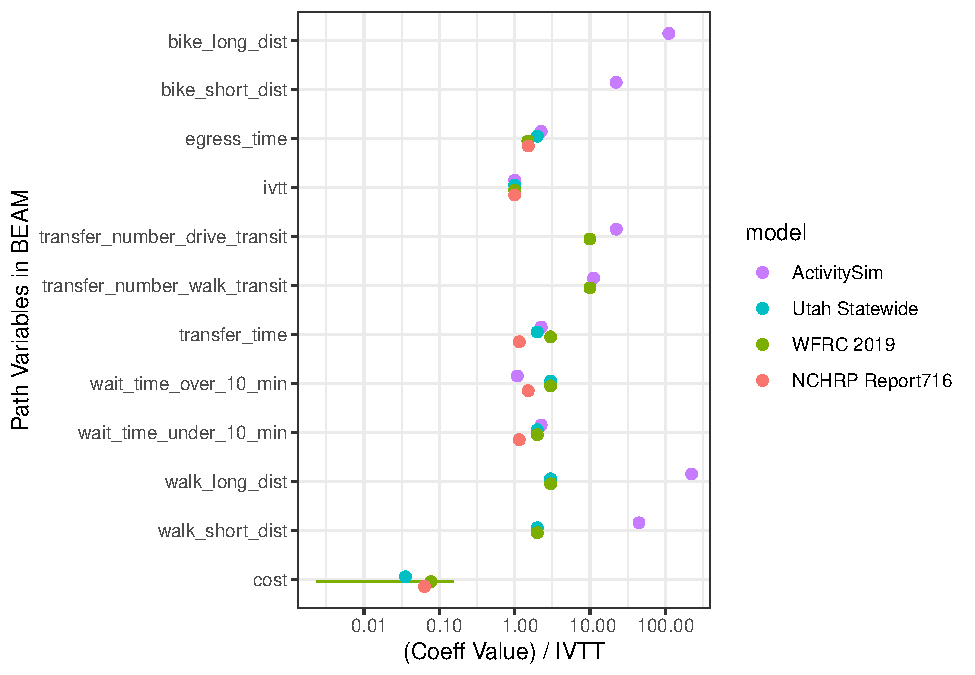
\includegraphics{thesis_files/figure-latex/hbw-1} 

}

\caption{Home-based work mode choice path coefficients model comparison.}\label{fig:hbw}
\end{figure}

Figure \ref{fig:hbs} shows the comparison of the path utility parameter values between all four models for home-based school trips. Similar to the home-based work analysis, for the egress time, ivtt, transfer time, and the wait times, ActivitySim seems to use a very similar coefficient value as the other three models. Again, the largest discrepancy exists with short and long walking distances. Since this is simply a difference between how walk distance is modeled, the discrepancy is ignored. In addition, the other three models did not have information on number of transfers. As a result, there is no comparison done with number of transfers. ActivitySim's path coefficient values do not require calibration for the home-based school parameters.

\begin{figure}

{\centering 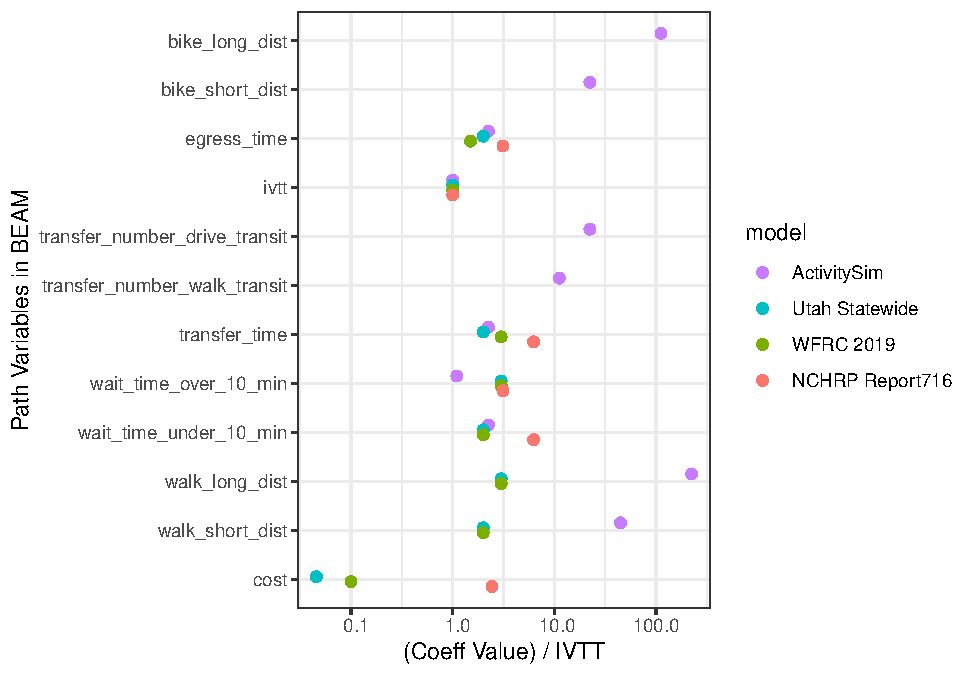
\includegraphics{thesis_files/figure-latex/hbs-1} 

}

\caption{Home-based school mode choice path coefficients model comparison.}\label{fig:hbs}
\end{figure}

Lastly, Figure \ref{fig:hbo} shows the comparison of path utility parameter values between all four models for home-based other trips. Again, besides for walk distance all variables seem to be similar between all four models. An interesting point is that for models other than ActivitySim, the cost coefficient varies greatly. Fortunately, ActivitySim bases the cost coefficient on each individual's value of time so this is not a concern. Overall, for all purpose types the coefficients used by ActivitySim are similar enough to other models that exist, and therefore do not require calibration. The ActivitySim alternative specific constants do, however, require calibration (See Section \ref{clib}).

\begin{figure}

{\centering 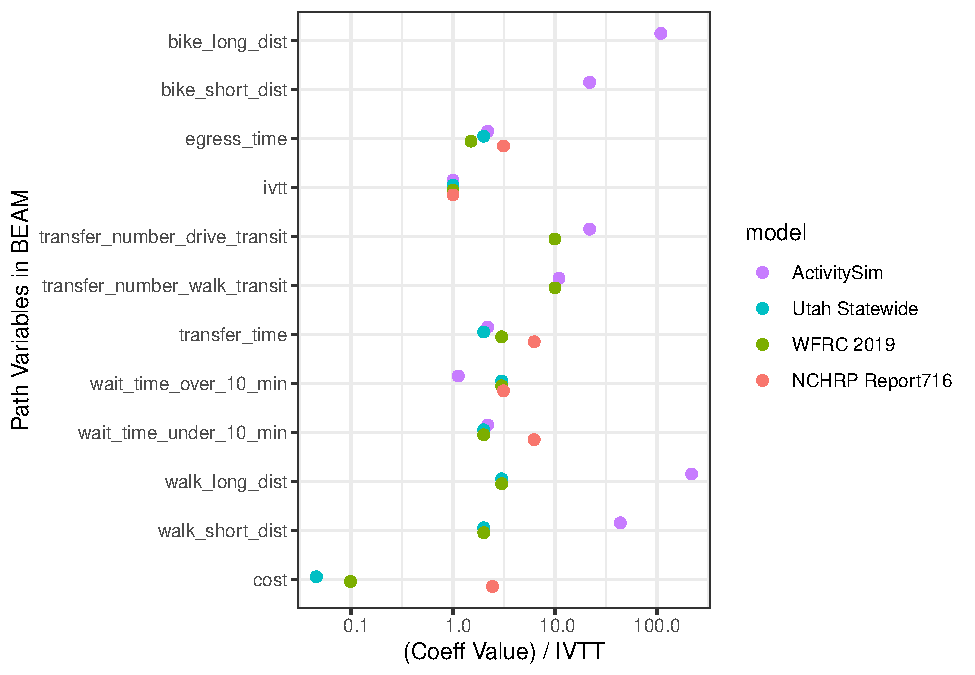
\includegraphics{thesis_files/figure-latex/hbo-1} 

}

\caption{Home-based other mode choice path coefficients model comparison.}\label{fig:hbo}
\end{figure}

\hypertarget{clib}{%
\subsection{Mode Choice Calibration}\label{clib}}

\hypertarget{summary}{%
\section{Summary}\label{summary}}

\hypertarget{results}{%
\chapter{Results}\label{results}}

\hypertarget{total-modal-distribution}{%
\section{Total Modal Distribution}\label{total-modal-distribution}}

\hypertarget{path-person-and-location-analysis}{%
\section{Path, Person, and Location Analysis}\label{path-person-and-location-analysis}}

\hypertarget{subtour-trip-analysis}{%
\section{Subtour Trip Analysis}\label{subtour-trip-analysis}}

\hypertarget{discussion}{%
\chapter{Discussion}\label{discussion}}

\hypertarget{conclusions}{%
\chapter{Conclusions}\label{conclusions}}

`r
\# \{=latex\} for thesis
\# \{\} for elsevier'

\cleardoublepage
    \bookmarksetupnext{level=part}
    \phantomsection
    \addcontentsline{toc}{chapter}{References}
    \begin{centering}
    REFERENCES\\
    \vskip 1 \baselineskip
    \end{centering}
    

\hypertarget{refs}{}
\begin{CSLReferences}{1}{0}
\leavevmode\vadjust pre{\hypertarget{ref-asim}{}}%
ActivitySim. 2021. \emph{ActivitySim: An Open Platform for Activity-Based Travel Modeling} (version 0.9.9.1). \url{https://github.com/ActivitySim/activitysim.}

\leavevmode\vadjust pre{\hypertarget{ref-agrc}{}}%
AGRC. 2021. \emph{Automated Geographic Reference Center}. \url{https://gis.utah.gov/}.

\leavevmode\vadjust pre{\hypertarget{ref-beam}{}}%
BEAM. 2022. \emph{Behavior, Energy, Autonomy, and Mobility}. Lawrence Berkeley National Laboratory the UC Berkeley Institute for Transportation Studies. \url{https://beam.readthedocs.io/en/develop/users.html}.

\leavevmode\vadjust pre{\hypertarget{ref-biehl19}{}}%
Biehl, Alec, Alireza Ermagun, and Amanda Stathopoulos. 2019. {``Utilizing Multi-Stage Behavior Change Theory to Model the Process of Bike Share Adoption.''} \emph{Transport Policy} 77: 30--45.

\leavevmode\vadjust pre{\hypertarget{ref-bowman98}{}}%
Bowman, John Lawrence. 1998. {``The Day Activity Schedule Approach to Travel Demand Analysis.''} PhD thesis, Massachusetts Institute of Technology.

\leavevmode\vadjust pre{\hypertarget{ref-nchrp}{}}%
Cambridge Systematics, Inc., Inc. Vanasse Hangen Brustlin, Gallop Corporation, Chandra R. Bhat, LLC Shapiro Transportation Consulting, and PLLC Martin/Alexiou/Bryson. 2012. {``Travel Demand Forecasting: Parameters and Techniques.''} In \emph{NCHRP Report 716}, 55--60. Transportation Research Board.

\leavevmode\vadjust pre{\hypertarget{ref-campbell16}{}}%
Campbell, Andrew A, Christopher R Cherry, Megan S Ryerson, and Xinmiao Yang. 2016. {``Factors Influencing the Choice of Shared Bicycles and Shared Electric Bikes in Beijing.''} \emph{Transportation Research Part C: Emerging Technologies} 67: 399--414.

\leavevmode\vadjust pre{\hypertarget{ref-cho22}{}}%
Cho, Shin-Hyung, and DongHwa Shin. 2022. {``Estimation of Route Choice Behaviors of Bike-Sharing Users as First-and Last-Mile Trips for Introduction of Mobility-as-a-Service (MaaS).''} \emph{KSCE Journal of Civil Engineering}, 1--12.

\leavevmode\vadjust pre{\hypertarget{ref-r5}{}}%
Conveyal. 2022. \emph{R5: Rapid Realistic Routing on Real-World and Reimagined Networks}. \url{https://github.com/conveyal/r5}.

\leavevmode\vadjust pre{\hypertarget{ref-dean21}{}}%
Dean, Matthew D, and Kara M Kockelman. 2021. {``Spatial Variation in Shared Ride-Hail Trip Demand and Factors Contributing to Sharing: Lessons from Chicago.''} \emph{Journal of Transport Geography} 91: 102944.

\leavevmode\vadjust pre{\hypertarget{ref-dong20}{}}%
Dong, Xiaoxia. 2020. {``Trade Uber for the Bus?''} \emph{Journal of the American Planning Association} 86 (2): 222--35.

\leavevmode\vadjust pre{\hypertarget{ref-gomes21}{}}%
Gomes, Viviani Antunes, MUC CALDAS, and Cira Souza Pitombo. 2021. {``An Investigation of Trip-Chaining Behaviour Based on Activity Participation, Socioeconomic Variables and Aggregated Characteristics of Modal Alternatives.''} \emph{Revista Transportes} 29 (1): 21--41.

\leavevmode\vadjust pre{\hypertarget{ref-hasnine21}{}}%
Hasnine, Md Sami, and Khandker Nurul Habib. 2021. {``Tour-Based Mode Choice Modelling as the Core of an Activity-Based Travel Demand Modelling Framework: A Review of State-of-the-Art.''} \emph{Transport Reviews} 41 (1): 5--26. \url{https://doi.org/10.1080/01441647.2020.1780648}.

\leavevmode\vadjust pre{\hypertarget{ref-horl19b}{}}%
Hörl, Sebastian, Claudio Ruch, Felix Becker, Emilio Frazzoli, and Kay W Axhausen. 2019. {``Fleet Operational Policies for Automated Mobility: A Simulation Assessment for Zurich.''} \emph{Transportation Research Part C: Emerging Technologies} 102: 20--31.

\leavevmode\vadjust pre{\hypertarget{ref-hosseinzadeh21}{}}%
Hosseinzadeh, Aryan, Majeed Algomaiah, Robert Kluger, and Zhixia Li. 2021. {``Spatial Analysis of Shared e-Scooter Trips.''} \emph{Journal of Transport Geography} 92: 103016.

\leavevmode\vadjust pre{\hypertarget{ref-hyland18}{}}%
Hyland, Michael, Zihan Hong, Helen Karla Ramalho de Farias Pinto, and Ying Chen. 2018. {``Hybrid Cluster-Regression Approach to Model Bikeshare Station Usage.''} \emph{Transportation Research Part A: Policy and Practice} 115: 71--89.

\leavevmode\vadjust pre{\hypertarget{ref-kang21}{}}%
Kang, Shuqing, Aupal Mondal, Aarti C Bhat, and Chandra R Bhat. 2021. {``Pooled Versus Private Ride-Hailing: A Joint Revealed and Stated Preference Analysis Recognizing Psycho-Social Factors.''} \emph{Transportation Research Part C: Emerging Technologies} 124: 102906.

\leavevmode\vadjust pre{\hypertarget{ref-knapen21}{}}%
Knapen, Luk, Muhammad Adnan, Bruno Kochan, Tom Bellemans, Marieke van der Tuin, Han Zhou, and Maaike Snelder. 2021. {``An Activity Based Integrated Approach to Model Impacts of Parking, Hubs and New Mobility Concepts.''} \emph{Procedia Computer Science} 184: 428--37.

\leavevmode\vadjust pre{\hypertarget{ref-nate}{}}%
Lant, Nathan John. 2021. {``Estimation and Simulation of Daily Activity Patterns for Individuals Using Wheelchairs.''} PhD thesis, Brigham Young University.

\leavevmode\vadjust pre{\hypertarget{ref-lazarus20}{}}%
Lazarus, Jessica, Jean Carpentier Pourquier, Frank Feng, Henry Hammel, and Susan Shaheen. 2020. {``Micromobility Evolution and Expansion: Understanding How Docked and Dockless Bikesharing Models Complement and Compete--a Case Study of San Francisco.''} \emph{Journal of Transport Geography} 84: 102620.

\leavevmode\vadjust pre{\hypertarget{ref-leeb21}{}}%
Lee, Hyukseong, Kwangho Baek, Jin-Hyuk Chung, and Jinhee Kim. 2021. {``Factors Affecting Heterogeneity in Willingness to Use e-Scooter Sharing Services.''} \emph{Transportation Research Part D: Transport and Environment} 92: 102751.

\leavevmode\vadjust pre{\hypertarget{ref-lee21}{}}%
Lee, Mina, Joseph YJ Chow, Gyugeun Yoon, and Brian Yueshuai He. 2021. {``Forecasting e-Scooter Substitution of Direct and Access Trips by Mode and Distance.''} \emph{Transportation Research Part D: Transport and Environment} 96: 102892.

\leavevmode\vadjust pre{\hypertarget{ref-li18b}{}}%
Li, Qing, Feixiong Liao, Harry JP Timmermans, Haijun Huang, and Jing Zhou. 2018. {``Incorporating Free-Floating Car-Sharing into an Activity-Based Dynamic User Equilibrium Model: A Demand-Side Model.''} \emph{Transportation Research Part B: Methodological} 107: 102--23.

\leavevmode\vadjust pre{\hypertarget{ref-li18}{}}%
Li, Weibo, and Maria Kamargianni. 2018. {``Providing Quantified Evidence to Policy Makers for Promoting Bike-Sharing in Heavily Air-Polluted Cities: A Mode Choice Model and Policy Simulation for Taiyuan-China.''} \emph{Transportation Research Part A: Policy and Practice} 111: 277--91.

\leavevmode\vadjust pre{\hypertarget{ref-li20}{}}%
Li, Yuanyuan, Yang Liu, and Jun Xie. 2020. {``A Path-Based Equilibrium Model for Ridesharing Matching.''} \emph{Transportation Research Part B: Methodological} 138: 373--405.

\leavevmode\vadjust pre{\hypertarget{ref-macfarlane21}{}}%
Macfarlane, Gregory S, Nathan J Lant, et al. 2021. {``Estimation and Simulation of Daily Activity Patterns for Individuals Using Wheelchairs.''} Utah. Dept. of Transportation. Division of Research.

\leavevmode\vadjust pre{\hypertarget{ref-mahmoudi21}{}}%
Mahmoudi, Monirehalsadat, Lu (Carol) Tong, Venu M. Garikapati, Ram M. Pendyala, and Xuesong Zhou. 2021. {``How Many Trip Requests Could We Support? An Activity-Travel Based Vehicle Scheduling Approach.''} \emph{Transportation Research Part C: Emerging Technologies} 128. https://doi.org/\url{https://doi.org/10.1016/j.trc.2021.103222}.

\leavevmode\vadjust pre{\hypertarget{ref-mckenzie19}{}}%
McKenzie, Grant. 2019. {``Spatiotemporal Comparative Analysis of Scooter-Share and Bike-Share Usage Patterns in Washington, DC.''} \emph{Journal of Transport Geography} 78: 19--28.

\leavevmode\vadjust pre{\hypertarget{ref-mo22}{}}%
Mo, Dong, Xiqun Michael Chen, and Junlin Zhang. 2022. {``Modeling and Managing Mixed on-Demand Ride Services of Human-Driven Vehicles and Autonomous Vehicles.''} \emph{Transportation Research Part B: Methodological} 157: 80--119.

\leavevmode\vadjust pre{\hypertarget{ref-mtc12}{}}%
MTC. 2012. \emph{Travel Model Development: Calibration and Validation Technical Report}. Metropolitan Transportation Commission with Parsons Brinckerhoff, Inc.

\leavevmode\vadjust pre{\hypertarget{ref-muhammad19}{}}%
Muhammad, Hafiz, Ahsan IQBAL, Muhammad ADNAN, Bruno KOCHAN, Tom BELLEMANS, and Davy JANSSENS. 2019. {``Incorporating MaaS Concept into an Operational Activity-Based Modelling Platform.''} In.

\leavevmode\vadjust pre{\hypertarget{ref-nayak22}{}}%
Nayak, Suchismita, and Debapratim Pandit. 2022. {``Activity-Based Model: Requisite for a New Travel Demand Forecasting Approach for India.''} In \emph{Proceedings of the Fifth International Conference of Transportation Research Group of India}, 109--21. Springer.

\leavevmode\vadjust pre{\hypertarget{ref-nguyen22}{}}%
Nguyen, Tri K, Nam H Hoang, and Hai L Vu. 2022. {``A Unified Activity-Based Framework for One-Way Car-Sharing Services in Multi-Modal Transportation Networks.''} \emph{Transportation Research Part E: Logistics and Transportation Review} 157: 102551.

\leavevmode\vadjust pre{\hypertarget{ref-philip13}{}}%
Philip, Milimol, T Sreelatha, and Soosan George. 2013. {``Activity Based Travel Behavioural Study and Mode Choice Modelling.''} \emph{Int J Innov Res Sci Eng Technol} 2 (1): 181--90.

\leavevmode\vadjust pre{\hypertarget{ref-popsim}{}}%
PopulationSim. 2021. \emph{An Open Platform for Population Synthesis} (version 0.5). \url{https://activitysim.github.io/populationsim/}.

\leavevmode\vadjust pre{\hypertarget{ref-reck21}{}}%
Reck, Daniel J, He Haitao, Sergio Guidon, and Kay W Axhausen. 2021. {``Explaining Shared Micromobility Usage, Competition and Mode Choice by Modelling Empirical Data from Zurich, Switzerland.''} \emph{Transportation Research Part C: Emerging Technologies} 124: 102947.

\leavevmode\vadjust pre{\hypertarget{ref-rsg16}{}}%
RSG. 2016. \emph{Pricing and Travel Time Reliability Enhancements in the SANDAG Activity-Based Travel Model: Final Report}.

\leavevmode\vadjust pre{\hypertarget{ref-sanchez19}{}}%
Sánchez, Pedro, Denis Pato, Gabriel Martín, et al. 2019. {``CTRANSPORT: Multi-Agent-Based Simulation.''}

\leavevmode\vadjust pre{\hypertarget{ref-shimizu13}{}}%
Shimizu, Shota, Kenju Akai, and Nariaki Nishino. 2013. {``Modeling and Multi-Agent Simulation of Bicycle Sharing.''} In \emph{International Conference on Serviceology}, 39--46. Springer.

\leavevmode\vadjust pre{\hypertarget{ref-song19}{}}%
Song, Mingzhu, Yi Zhang, Zuojun Max Shen, Meng Li, and Zhenning Dong. 2019. {``Mode Shift from Car to Bike Shared: A Travel-Mode Choice Model.''} In \emph{CICTP 2019}, 2398--2410.

\leavevmode\vadjust pre{\hypertarget{ref-tuli21}{}}%
Tuli, Farzana Mehzabin, Suman Mitra, and Mariah B Crews. 2021. {``Factors Influencing the Usage of Shared e-Scooters in Chicago.''} \emph{Transportation Research Part A: Policy and Practice} 154: 164--85.

\leavevmode\vadjust pre{\hypertarget{ref-tzouras22}{}}%
Tzouras, Panagiotis G, Lambros Mitropoulos, Eirini Stavropoulou, Eleni Antoniou, Katerina Koliou, Christos Karolemeas, Antonis Karaloulis, et al. 2022. {``Agent-Based Models for Simulating e-Scooter Sharing Services: A Review and a Qualitative Assessment.''} \emph{International Journal of Transportation Science and Technology}.

\leavevmode\vadjust pre{\hypertarget{ref-utahstate}{}}%
UDOT. 2021. \emph{Utah State Travel Demand Model}. Utah Department of Transportation.

\leavevmode\vadjust pre{\hypertarget{ref-gtfs}{}}%
UTA. 2021. {``OpenMobilityData - GTFS.''} Utah Transit Authority. \url{https://transitfeeds.com/p/utah-transportation-authority/59}.

\leavevmode\vadjust pre{\hypertarget{ref-vyas19}{}}%
Vyas, Gaurav, Pooneh Famili, Peter Vovsha, Daniel Fay, Ashish Kulshrestha, Greg Giaimo, and Rebekah Anderson. 2019. {``Incorporating Features of Autonomous Vehicles in Activity-Based Travel Demand Model for Columbus, OH.''} \emph{Transportation} 46 (6): 2081--2102.

\leavevmode\vadjust pre{\hypertarget{ref-wadud21}{}}%
Wadud, Zia, and Phani Kumar Chintakayala. 2021. {``To Own or Not to Own--That Is the Question: The Value of Owning a (Fully Automated) Vehicle.''} \emph{Transportation Research Part C: Emerging Technologies} 123: 102978.

\leavevmode\vadjust pre{\hypertarget{ref-welch20}{}}%
Welch, Timothy F, Steven R Gehrke, and Alyas Widita. 2020. {``Shared-Use Mobility Competition: A Trip-Level Analysis of Taxi, Bikeshare, and Transit Mode Choice in Washington, DC.''} \emph{Transportmetrica A: Transport Science} 16 (1): 43--55.

\leavevmode\vadjust pre{\hypertarget{ref-wfrc}{}}%
WFRC. 2019. \emph{Wasatch Front Travel Demand Model} (version v8.3.1). Wasatch Front Regional Council. \url{https://wfrc.org/programs/models-forecasting/}.

\leavevmode\vadjust pre{\hypertarget{ref-xu19}{}}%
Xu, Xiang, Hani S Mahmassani, and Ying Chen. 2019. {``Privately Owned Autonomous Vehicle Optimization Model Development and Integration with Activity-Based Modeling and Dynamic Traffic Assignment Framework.''} \emph{Transportation Research Record} 2673 (10): 683--95.

\leavevmode\vadjust pre{\hypertarget{ref-younes20}{}}%
Younes, Hannah, Zhenpeng Zou, Jiahui Wu, and Giovanni Baiocchi. 2020. {``Comparing the Temporal Determinants of Dockless Scooter-Share and Station-Based Bike-Share in Washington, DC.''} \emph{Transportation Research Part A: Policy and Practice} 134: 308--20.

\leavevmode\vadjust pre{\hypertarget{ref-zhang21}{}}%
Zhang, Wenwen, Ralph Buehler, Andrea Broaddus, and Ted Sweeney. 2021. {``What Type of Infrastructures Do e-Scooter Riders Prefer? A Route Choice Model.''} \emph{Transportation Research Part D: Transport and Environment} 94: 102761.

\leavevmode\vadjust pre{\hypertarget{ref-zhou20}{}}%
Zhou, Fan, Zuduo Zheng, Jake Whitehead, Simon Washington, Robert K Perrons, and Lionel Page. 2020. {``Preference Heterogeneity in Mode Choice for Car-Sharing and Shared Automated Vehicles.''} \emph{Transportation Research Part A: Policy and Practice} 132: 633--50.

\leavevmode\vadjust pre{\hypertarget{ref-zhou19}{}}%
Zhou, Xiaolu, Mingshu Wang, and Dongying Li. 2019. {``Bike-Sharing or Taxi? Modeling the Choices of Travel Mode in Chicago Using Machine Learning.''} \emph{Journal of Transport Geography} 79: 102479.

\leavevmode\vadjust pre{\hypertarget{ref-zuniga22}{}}%
Zuniga-Garcia, Natalia, Mauricio Tec, James G Scott, and Randy B Machemehl. 2022. {``Evaluation of e-Scooters as Transit Last-Mile Solution.''} \emph{Transportation Research Part C: Emerging Technologies} 139: 103660.

\end{CSLReferences}


% Index?

\end{document}
